\documentclass[]{report}
\usepackage[utf8x]{inputenc}
\usepackage{graphicx}
\usepackage{amsmath}
\usepackage{amssymb}
\usepackage{tikz}
\usepackage{todonotes}
\usepackage[outdir=./]{epstopdf}
\usepackage{pgfplots}
\usepackage{epstopdf}
\usepackage{listings}
\usepackage{circuitikz}
\usepackage{float}
\usepackage{cite}
\usepackage{cleveref}
\usepackage{ragged2e} % For text alignment


\newenvironment{custom_itemize}{
\begin{itemize}
  \setlength{\itemsep}{0pt}
  \setlength{\parskip}{0pt}
  \setlength{\parsep}{0pt}
}{\end{itemize}}


\usepackage[hmarginratio=1:1,top=22mm,columnsep=16pt]{geometry} % Document margins
%\usepackage{multicol} % Used for the two-column layout of the document


%\usepackage{bm}


\title{Lidar sensor for Europa Clipper feasability study}
\author{Kees Kroep}


\begin{document}
%  \twocolumn[{%
% \begin{@twocolumnfalse}
  \maketitle
%   \end{@twocolumnfalse}
% }]


\section*{Abstract}
This document investigates the feasability of a lidar sensor based of performance requirements provided by NASA. The main focus of this study is both the required laser power and the resilience of the device against proton radiation. Other considerations include manufacturability, readout specifications and lens specifications. Based on the results of this study a design will be proposed. A radiation test is performed to increase the knowledge about the radiation resilience of the technology used in the proposed design. Based on these findings a design is proposed.

%\clearpage
\tableofcontents
\clearpage

\section*{Introduction}
The Europa Clipper is a planned mission by NASA  to conduct  detailed reconnaissance of Juliter;s moon Europa and investigate whether the moon could harbor condition suitable for life. To aid in the landing process, a lidar sensor is proposed. The functionaily of the lidar sensor is twofold. At hig altitudes, the Lidar sensor must operate in Altimetry Mode, and be capable to accurately measure the altitude of the device with respect to the surface of Europa. When the Europa Clipper gets closer to Europa, the lidar sensor must switch to a Hazard Detection Mode, where it scans the landing site on the surface of Europa to make a heightmap to pick a suitable landing spot and to aid the final stages of the landing process.

This study will investigate the feasability of such a lidar sensor. The focus will lie on required laser power to meet the required resollution, and the resilience of the device against proton irradiation. 

\Cref{sec:requirements_and_specifications} will state the relevant specifications as provided by NASA, and elaborate on the basic structure of the lidar sensor. Finally all assumptions used throughout the study will be listed. \Cref{sec:altimetry_mode} will investigate design choices for the Altimetry Mode and make perdictions about the feasability of the proposed design. \Cref{sec:hazard_detection_mode} will investigate design choices for the Hazaerd Detection Mode, with a larger emphasis on SPAD design and manufacturability. \Cref{sec:radiation} will investigate the resilience against proton irradiation of the proposed technology by performing a radiation test with a proton beam. Finally \cref{sec:specs} will summarize the study and list a preliminary specsheet for the proposed design.

\chapter{Requirements and Specifications}\label{sec:requirements_and_specifications}
\section{High level specifications} 
\label{sec:high_level_specifications}
The radiation and mass, power and volume budget are listed in \cref{tab:req_radiation} and \cref{tab:req_mpv}.

\begin{table}[H]
\centering
\caption{Overview of radiation limitations}
\label{tab:req_radiation}
\begin{tabular}{|l|l|}
\hline
\textbf{Radiation}      &          \\ \hline
\begin{tabular}[c]{@{}l@{}}Total Integrated Dose in Silicon\\     behind 100 mil Al spherical shell\end{tabular} & 500 krad \\ \hline
\end{tabular}
\end{table}

\begin{table}[H]
\centering
\caption{Requirements for mass, power and volume}
\label{tab:req_mpv}
\begin{tabular}{|l|l|} \hline
\textbf{Mass, Power \& Volume Budget}                                 &               \\ \hline
Optical Head                                                 & \textless5 kg \\
Inside vault                                                 & \textless1 kg \\
\begin{tabular}[c]{@{}l@{}}Max cable length between \\ 
optical head and electronics\end{tabular} & 2 m           \\
Power                                                        & \textless50 W \\ \hline
\end{tabular}
\end{table}

The Lidar sensor features two operation modes: the Altimetry Mode, and the Hazard Detection Mode. 

\subsection{Altimetry Mode} 
\label{ssec:altimetry_mode}

Altimetry Mode is the first phase of the landing. During the Altimetry Mode, the Lidar sensor has to provide the altitude of the sensor in relationship to the surface op Europa. The requirements for the Altimetry Mode are listed in \cref{tab:req_altimetry}

\begin{table}[H]
\centering
\caption{Requirements for Altimetry Mode}
\label{tab:req_altimetry}
\begin{tabular}{|l|ll|} \hline
\textbf{Altimetry Mode}     & Threshold & Goal   \\ \hline
Max acquisition Slant Range & 5 km      & 8 km   \\
Range Accuracy (3-sigma)    & 1\%       & 0.10\% \\
Update Rate                 & 0.1 Hz    & 1 Hz   \\ \hline
\end{tabular}
\end{table}

\subsection{Hazard Detection Mode} 
\label{ssec:hazard_detection_mode}

During the Hazard Detection Mode a 3d map of the surface of Europa must be created around the landing place. The Hazard Mode is operational when the sensor is close enough to the surface of Europa. The requirements for the Hazard Detection Mode can be found in \cref{tab:req_hazard_detection}

\begin{table}[H]
\centering
\caption{Requirements for Hazard Detection Mode}
\label{tab:req_hazard_detection}
\begin{tabular}{|l|ll|} \hline
\textbf{Hazard Detection Mode}               & Threshold     & Goal          \\ \hline
Max range (altitude)                         & 400 m         & 500 m         \\
Min Operational Range (altitude)             & 5 m           & 1 m           \\
Range Accurcay (3-sigma on final 3D map)     & 10 cm         & 5 cm          \\
Ground Sample Distance (per pixel on 3D map) & 10 cm         & 5 cm          \\
Ground Area Coverage at max altitude         & 100 m x 100 m & 125 m x 125 m \\
Time for 3D map creation                     & 1 s           & 1 s           \\ \hline
\end{tabular}
\end{table}

%\section{System engineering level design} 
\label{sec:system_engineering_level_design}
In this section a system engineering level design is constructed that meets the performance requirements stated in \cref{sec:high_level_specifications}. \Cref{ssec:overview} shall provide an overview of the system, \cref{ssec:assumptions} shall list the assumptions made, and \cref{ssec:trade_offs_and_methodology} shall elaborate on trade-offs and design decisions. 

\section{Overview} 
\label{ssec:overview}
A schematic overview of the sensor is shown in \cref{tkz:schematic_overview}.

\begin{figure}[H]
    \centering



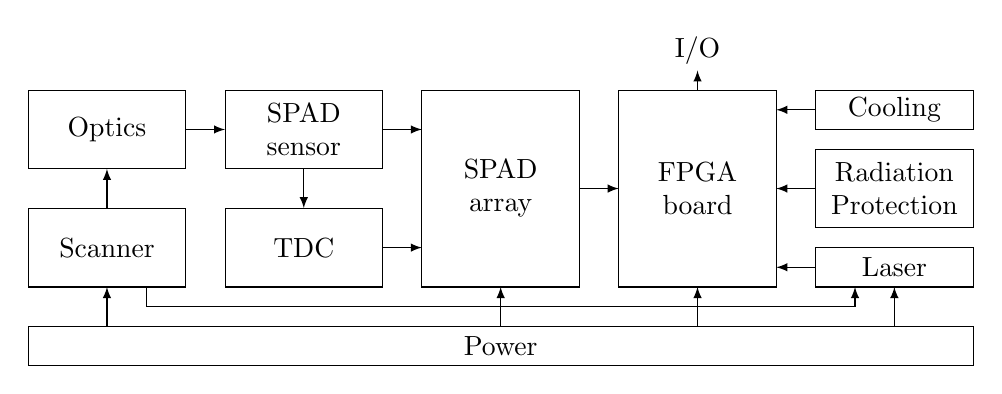
\begin{tikzpicture}[scale=.5]

\draw  (13,2) rectangle (17,1) node[pos=.5, align=center]{Cooling};
\draw  (13,0.5) rectangle (17,-1.5) node[pos=.5, align=center]{Radiation\\Protection};
\draw  (-7,-4) rectangle (17,-5) node[pos=.5, align=center]{Power};
\draw  (13,-2) rectangle (17,-3) node[pos=.5, align=center]{Laser};
\draw  (8,2) rectangle (12,-3) node[pos=.5, align=center]{FPGA\\board};
\draw  (3,2) rectangle (7,-3) node[pos=.5, align=center]{SPAD\\array};
\draw  (-2,2) rectangle (2,0) node[pos=.5, align=center]{SPAD\\sensor};
\draw  (-7,2) rectangle (-3,0) node[pos=.5, align=center]{Optics};
\draw  (-7,-1) rectangle (-3,-3) node[pos=.5, align=center]{Scanner};
\draw  (-2,-1) rectangle (2,-3) node[pos=.5, align=center]{TDC};

\draw [>=latex, ->](0,0) -- (0,-1);
\draw [>=latex, ->](2,-2) -- (3,-2);
\draw [>=latex, ->](13,1.5) -- (12,1.5);
\draw [>=latex, ->](7,-.5) -- (8,-.5);
\draw [>=latex, ->](2,1) -- (3,1);
\draw [>=latex, ->](13,-2.5) -- (12,-2.5);
\draw [>=latex, ->](10,2) -- (10,2.5);
\draw [>=latex, ->](-3,1) -- (-2,1);
\draw [>=latex, ->](13,-.5) -- (12,-.5);
\draw [>=latex, ->](5,-4) -- (5,-3);
\draw [>=latex, ->](10,-4) -- (10,-3);
\draw [>=latex, ->](15,-4) -- (15,-3);
\draw [>=latex, ->](-5,-1) -- (-5,0);
\node at (10,3) {I/O};

\draw [>=latex, ->](-5,-4) -- (-5,-3);
\draw [>=latex, ->](-4,-3) -- (-4,-3.5) -- (14,-3.5) -- (14,-3);

\end{tikzpicture}




    \caption{Schematic overview}
    \label{tkz:schematic_overview}
\end{figure}

~\\
\textbf{Laser}: The laser must send short pulses but powerful pulses at a predefined frequency, to transmit photons that can be detected by the SPAD Sensor. A critical requirement for the laser is the amount of photons it is able to transmit as a function of time, within the budget and technical limitations. \\
\\
\textbf{SPAD Sensor}: The Single Photon Avalanche Diode (SPAD) is responsible for generating a digital pulse when hit by a photon. A circuit build around the SPAD must ensure that the SPAD is quenched as quickly as possible to minimize the deadline. A critical requirement for the SPAD is a small jitter to maximize the accuracy of the sensor.  \\
\\
\textbf{TDC}: The Time Interval to Digital Converter (TDC) is connected to the laser and the SPAD Sensor. The TDC must measure the time difference between the transmission of the laser and the receiving at the SPAD sensor. This measurement requires an accuracy of tens of picoseconds to meet the accuracy requirements.\\
\\
\textbf{Scanner}: The scanner handles the scanning motion that is needed to accumulate the entire picture. Different scanning motions can introduce undesired jitter and heavily influence the amount of SPAD Sensors that are needed on teh SPAD Array. \\
\\
\textbf{SPAD Array}: The SPAD Array integrates the SPAD Sensors on a chip and connects them to the TDCs. The layout of the SPAD Array is closely related to the scanning motion that is used in the scanner.\\
\\
\textbf{Optics}:
The optics must transfer as much of the incoming photons as possible to the sensitive area on the SPAD Sensors. The Optics part also implements a bandpass filter around the target frequency. \\
\\
\textbf{FPGA Board}:
The FPGA Board controls the sensor. It is responsible for accumulating and interpreting the measurements from the TDCs, and controlling the Scanner and Laser. \\
\\
\textbf{Cooling}:
The cooling has to keep the temperature of the FPGA chip under a threshold temperature.\\
\\
\textbf{Radiation Protection}:
The Radiation Protection shields sensitive parts of the sensor from radiation. The most sensitive part of the system is expected to be the FPGA Board, based on experience.\\
\\
\textbf{Power}:
The power block has to supply the scanner, SPAD Array, FPGA Board, and the laser with the required power. The power block has to operate within the specified power budget.












\clearpage
\section{Assumptions} 
\label{ssec:assumptions}
This section will list the assumption that are made throughout the study.\\
\\
\textbf{Reflectivity of surface Europa}: It is assumed that out of all light that hit's Europa, $35\%$ is reflected in a perfectly diffuse manner.\\ 
\\
\textbf{Wavelength laser}: The wavelength of light emitted by the laser is assumed to be $850\,nm$. This wavelength is a typcial choice for Silicon SPAD's. The main reason for this wavelength as opposed to $550\,nm$ is because the that sunlight is less strong in that region, and less background noise will lft after applying a narrow bandpass filter. \\
\\
\textbf{Bandpass filter}:A bandpass filter will be used o filter background noise. This filter is assumed to be a bandpass filter with a center frequency of $850\,nm$ and a FWHM of $10\,nm$.The minimum transmission of the filter is $50\%$. These values are directly taken from the "\textit{850nm, 10nm FWHM, 12.5mm Mounted Diameter}" product made by Edmund Optics and sold for $75\,\$$.\\
\\
\textbf{Jitter of SPAD Sensor}: The jitter of the SPAD Sensor, or Full Width Half Max (FWHM) is assumed to be $100\,ps$. This value is a typical FWHM for state of the art Silicon SPAD's. \\
\\
\textbf{Jitter of TDC}: The jitter of the TDC's is assumed to be insignificant when compared to the jitter of $100\,ps$ caused by the SPAD Sensors. Experience with previous designs show that TDC jitter is generally a very small contributor to overall jitter.\\
\\
\textbf{Resolution of TDC}: The accuracy of the TDC is assumed to be $50\,ps$.\\
\\
\textbf{Sunlight}: It is assumed that the light from the sun that is reflected of Europa is the only signifant contributor to background noise. No other sources of light will be considered. \\
\\
\textbf{Photon Detection Probability}: It is assumed that the PDP of the SPADs is $10\%$.\\
\\
\textbf{Laser light hitting target}: It is assumed that all the light that leaves the laser is hitting the target area on Europa.
\\
\\
\textbf{Laser efficiency}: It is assumed that the laser has an efficiency of $10\%$.


\clearpage
\subsection{Trade-offs and Methodology} 
\label{ssec:trade_offs_and_methodology}
This section will list the trade-offs that can be found in the system. Each trade-off will be analyzed, and based on that, a decision will be made.


\subsubsection{High Frequency vs Low Frequency pulses}\label{sssec:high_low_freq}
The pulse frequency is limited by the roundtrip time  of the transmitted photons. The roundtrip time can be calculated using \cref{eq:roundtrip}

\begin{align}\label{eq:roundtrip}
t_{round} = \frac{2r}{c}
\end{align}
where $c\approx 3\cdot10^8$ is the speed of light, and $r$ the altitude of the sensor. The maximum pulse frequency can then be calculated using \cref{eq:pulse_f}

\begin{align}\label{eq:pulse_f}
f_{pulse} = \frac{1}{t_{round}} = \frac{c}{2r}
\end{align}

The maximum altitude are different for the Altimetry and Hazard Detection mode. The maximum pulse frequency of both modes is shown in \cref{tab:pulse_frequency}.

\input{tab/pulse_frequency_tab}

In order to increase the frequency, it is intersting to see what happens if the frequency is increased. The TDC measures the time between the last outgoing pulse and the incomming pulse. This means that the performed measurement $t_{TDC}$ can be calculated using \cref{eq:t_TDC_ToF}.

\begin{align}\label{eq:t_TDC_ToF}
	t_{TDC} &=ToF \mod T_{pulse}\\	
	ToF &= t_{TDC}+k\cdot T_{pulse} & k \in \mathbb{N}\label{eq:ToF_t_TDC}
\end{align}

 where $t_{TDC}$ is the measurement of the TDC, $ToF$ the time of flight, and $T_{pulse}$ the time period of the laser pulses. The returned answer is related to $ToF$ as shown in \cref{eq:ToF_t_TDC}. The precision of the measurement is maintained,  but on a larger scale the information is lost. \\
 \\
To solve this problem one can make measurements in two different frequencies. The idea is also applied in TDCs (Name of technique?), where two ring oscillators with different frequencies are used to amplify the range of the TDC. A similar idea can be applied here, but instead of using two oscillators, the time is devided in half, and in the first half the laser sends pulses in frequency $f_1$, and in the second half pulses with frequncy $f_2$. These two different measurements can first be used to determine the large scale ToF, and then the measurements can be combined to get a high accuracy to accompany that.\\
\\
As a proof of concept. This idea is applied to the Altimetry Mode. It is assumed that a difference of $5\,ns$ between $\lambda_1$ and $\lambda_2$ is sufficient. Now using a maximum $ToF$ one can calculate that optimal two frequencies, such that $f1_>f_2$ and $f_2$ as high as possible. 

\begin{align}
 	\frac{50\mu}{5n} &= 10660\\ 
 	\sqrt{\frac{50\mu}{5n}} &\approx 103
 \end{align} 
 Now two coprime numbers in $\mathbb{N}$ around 103 are 103 and 104. The resulting frequencies are
 \begin{align}
 	T_1 &= 103\cdot5n = 515n\\
 	T_2 &= 104\cdot5n = 520n\\
 	f_1 &= \frac{1}{T_1} = 1.9417\,MHz\\
 	f_2 &= \frac{1}{T_1} = 1.9231\,MHz\\
 \end{align}
The pulse frequency increases by a factor 100. A matlab plot of the resulting system is shown in \cref{fig:frequency_hopping}, where the measurement values of the TDC are plotted against the $ToF$.


\begin{figure}[h]
    \centering
    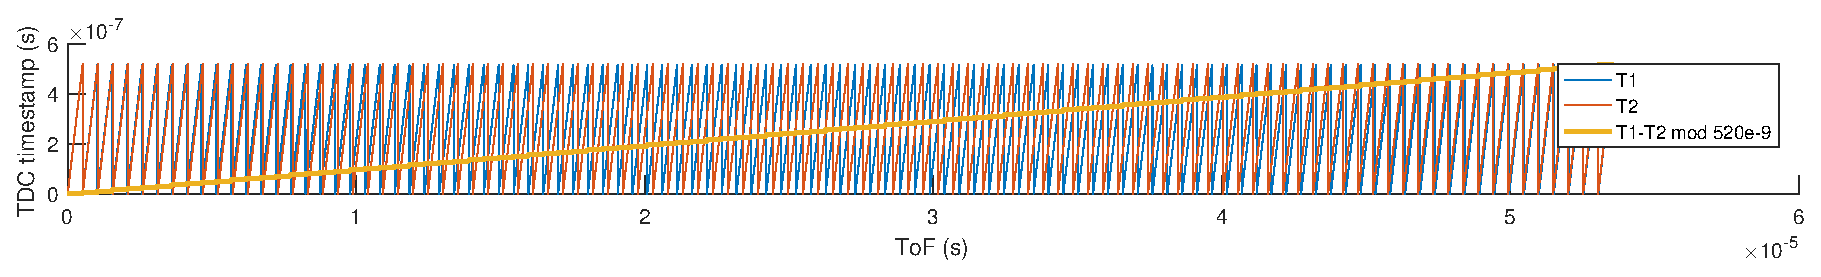
\includegraphics[width=\textwidth]{fig/frequency_hopping.eps}
    \caption{Matlab plot of TDC measurements vs ToF}
    \label{fig:frequency_hopping}
\end{figure}

The $ToF$ can be calculated using \cref{eq:ToF}.

\begin{align}
	t_{1-2} &= (t_1-t_2)\mod T_2\\
	ToF &= \frac{t_{1-2}}{T_2-T_1}T_1+\frac{t_1+t_2-t_{1-2}}{2}\label{eq:ToF}
\end{align}
where $t_1$ and $t_2$ are the timestamp measurements for $f_1$ and $f_2$ respectively. $t_{1-2}$ is the modulus of the time difference between $t_1$ and $t_2$.

\section{Optics}\label{ssec:optics}
The receiver optics are a good place to start of with, because the optics are not very dependent on results achieved in other areas. The optics have to transport as many desired photons, and as little unwanted photons to the active area on the SPADs as possible. All while having an acceptable depth of field. 

The most basic solution is a single lens with an aperture. The opacity of the lens can be calculated with the absorption of the lens material and f-number of the lens using \cref{eq:basic_opacity}.

\begin{align}\label{eq:basic_opacity}
\text{opacity} = \frac{1-\text{absorption}}{\text{f-number}^2}
\end{align}

 The performance of a possible configuration is shown in \cref{tab:basic_optics}

\input{tab/basic_optics_tab}

\subsection{Improvements}
There are a couple of additions that can improve the performance of the optics. The first and essential one, is the use of a bandpass filter. The transmitted signal will have a very specific bandwidth of $850\,nm$. Using a narrow bandpass filter one can filter out an enormous part of the background noise. The filter will have an opacity of $50\,\%$ for the target wavelength.

The captured photons that hit the lens need to be guided to the active area of the SPADs. If the active area on the chip is very small, one can use microlenses to improve the effectiveness of the optics. A Microlens focuses light on a single SPAD on the chip. Two types of microlenses will be considered: a spherical lens, and a square shaped lens. The presence of microlenses poses a limitation of the main lens. The f-number must be relatively large. A higher f-number means a smaller aperture and therefore more loss of photons. A way of dealing with this problem is to use a second lens instead. An overview of the available options is shown in \cref{tkz:receiver_optics}

\input{tkz/receiver_optics_tkz}

\begin{align}
\text{opacity} = (1-\text{absorption}_1)(1-\text{absorption}_2)\cdot\text{opacity filter}\cdot \frac{X}{\text{f-number}^2}
\end{align}
Where $X$ is the active area on the chip. A comparison between the different options is shown in \cref{tab:receiver_optics}

\input{tab/receiver_optics_tab}

The comparison in \cref{tab:receiver_optics} shows some good alternatives to the basic lens, if there is a need for it due to a small active area on the chip. However, most of the future calculations will focus on the basic model A.


\section{Scanning motion}\label{ssec:scanning_motion}
In \cref{ssec:SPADs}, it was concluded that a SPAD array with one SPAD per pixel is not feasible. Therefore a scanning motion is required. Possible scanning motions for different SPAD array configurations are shown in \cref{tkz:scanning_motions}. Note that the $2048\times1$ motion is in essence a special case of the $2048\times N$ motion, where exactly one row of pixels is observed at a time. The $M\times N$, with $M<2048$ and $N<2048$ needs a scanning motion in both $x$ and $y$ direction. This makes the scanning motion very complicated and unreliable. Therefore only the family of solutions with $2048\times N$ with $N<2048$ will be considered.


\input{tkz/scanning_motions_tkz}


\subsubsection{Background Noise}\label{ssec:background_noise}
For the background noise, it is assumed that the sun is the dominant source. The sum is modelled as an ideal black body. The spectral irradiance of the sun can be calculated using \cref{eq:spectral_irradiance}.
\begin{align}\label{eq:spectral_irradiance}
I_\lambda(\lambda,T) = \frac{2hc^2}{\lambda^5}\frac{1}{e^{\frac{hc}{\lambda kT}}-1}
\end{align}
where $I_\lambda(v,t)$ is spectral irradiance with unit $W/m^3$. \\
$h$ is the planck constant\\
$c$ is the speed of light in vacuum \\
$k$ is the Boltzman constant \\
$\lambda$ is the wavelength of the electromagnetic radiation\\
$T$ is the absolute temperature of the body\\
The spectral irradiance of the sun is calculated in \cref{tab:sun_irradiance}.

\input{tab/sun_irradiance_tab}

The next step is to calculate the power emitted by the sun in the specified bandwidth, at the location of Europa. This is done by modelling sun as a point source, and then spreading that power over a sphere with a radius equal to the distance between the sun and Europa, as is done in \cref{eq:point_source}.

\begin{align}\label{eq:point_source}
    P_{sun} = I_{\text{sun}} B_\lambda S \frac{r_{\text{sun}}^2}{r_{\text{europa}}^2}
\end{align}
where $I_{\text{sun}}$ is the spectral irradiance of the sun at the center frequency of the filter, $B_\lambda$ is the bandwidth of the filter in meters, $S$ the surface area of the target area on Europa, $r_{\text{sun}}$ the of radius of the sun, and $r_{\text{europa}}$ the distance between Europa and the sun. The effective radiance of the background noise at Europa is calculated in \cref{tab:power_background} using \cref{eq:point_source}.

\input{tab/effective_irradiance_tab}
\subsection{Resolution} 
\label{ssec:resolution}
The requirement for the altimetry mode changes based on the height. The target is a resolution of at least $0.1\,\%$. To ensure that this requirement is met, both the largest altitude of $8\,km$, and the smallest altitude of $500\,m$ will be investigated.

The minimum resolution for the largest and shortest altitude are $8\,m$ and $0.5\,m$ respectively. The maximum allowable FWHM can be calculated using \cref{eq:max_FWHM}.
 Using \cref{eq:FWHM_sigma} the maximum standard deviation can be calculated. The calculations are performed

\begin{align}\label{eq:max_FWHM}
FWHM_{max} = \frac{2x}{c}
\end{align}

\input{tab/AM_requirements_tab}







\subsubsection{standard deviation shortcut}
To calculate the standard deviation of the sum of multiple random variables that are independent and uncorrelated, one can use \cref{eq:variance_weighted_sum}


\begin{align}\label{eq:variance_weighted_sum}
\newcommand{\Var}{\mathrm{Var}}
 	\Var[aX+bY+cZ] = a^2\Var[X]+b^2\Var[Y]+c^2\Var[Z]
\end{align}




Next consider a situation where there are two random variable distributions. The first distribution is $S$, which is a normal distribution with $\mu_s=ToF$, where $ToF \in \{0, 50\mu\}$, and $\sigma_s=100p$. The second distribution is $N$, which is a uniform distribution with $\mu_n=\frac{50\mu}{2}$ and $\sigma_n=\frac{50\mu}{\sqrt{12}}$.

\begin{align}
	\mu_{mean} &= \frac{1}{110}\Big(\sum_{k=1}^{100}\mu_s+\sum_{l=1}^{10}\mu_n\Big)\\
			   &= \frac{100ToF+10*25\mu}{110}\\
			   &= \frac{10}{11}ToF+227.3n
\end{align}


\begin{align}
	\mathrm{Var}_{mean} &= \mathrm{Var}\Big[\frac{1}{110}\Big(\sum_{k=1}^{100}S_k+\sum_{l=1}^{10}N_l\Big)\Big]\\ 
	 &= \frac{1}{110^2}\Big(\sum_{k=1}^{100}\mathrm{Var}[S]+\sum_{l=1}^{10}\mathrm{Var}[N]\Big)\\
	&= \frac{1}{110^2}(100\sigma_s^2+10\sigma_n^2)\\
	&= \frac{10^{-18}+2.0833\cdot10^{-9}}{110^2}\\
	&= 1.7218\cdot10^{-13}\\
	\sigma_{mean} &= \sqrt{\mathrm{Var}_{mean}}\\
				  &= 414.94n
\end{align}



% Now we grab 100 samples out of $S$ and 10 out of $N$. First, the $\sigma$ and $\mu$ of the average of the 100 samples of $S$ is calculated.

% \begin{align}
% 	\mu_{s,mean} &= \frac{1}{100}\sum_{k=1}^{100}\mu_s\\
% 			     &= ToF
% \end{align}

% \begin{align}
% 	\mathrm{Var}[\frac{1}{100}\sum_{k=1}^{100}S_k] &= \frac{1}{100^2}\sum_{k=1}^{100} \mathrm{Var}[S_k]\\
% 						  &= \frac{\mathrm{Var}[S]}{100}\\
% 	\sigma_{s,mean} &= \frac{\sigma_s}{\sqrt{100}}\\
% 					&= 10p
% \end{align}

% Next the average of 10 samples of $N$ is calculated.

% \begin{align}
% 	\mu_{n,mean} &= \frac{1}{10}\sum_{k=1}^{10}\mu_n\\
% 			     &= 25\mu
% \end{align}

% \begin{align}
% 	\mathrm{Var}[\frac{1}{10}\sum_{k=1}^{10}] &= \frac{1}{10^2}\sum_{k=1}^{10} \mathrm{Var}[N_k]\\
% 						  &= \frac{\mathrm{Var}[N]}{10}\\
% 	\sigma_{s,mean} &= \frac{\sigma_n}{\sqrt{10}}\\
% 					&= \frac{50\mu}{\sqrt{120}}
% 					&\approx 4.5644\mu
% \end{align}

% Next the two resulting functions are combined






% \subsection{Laser}
The laser is responsible for the photons that are used for the Time of Flight (ToF) measurement. The laser has to ensure that the Signal to Background Noise Ratio (SBNR) is at least 0 dB. The power budget of the entire system is $50\,W$, which is the main bottleneck for the performance of the laser. The wavelength of the laser is $850\,nm$. The $P_B$ is already calculated in \cref{ssec:background_noise}. In order to achieve an SNR of 0 dB, the signal power $P_S$ must therefore at least match the background noise power that hits the surface of Europa. One can calculate the signal power at the optics using \cref{eq:P_S}.

\begin{align}\label{eq:P_S}
	P_S = P_{pulse} \cdot f_{pulse} \cdot R_{\text{Europa}}
\end{align}
where $P_{pulse}$ is the power of a single pulse of the laser, $f_{pulse}$ the frequency at which the pulses are transmitted, $R_{\text{Europa}}$ the reflectivity of Europa, and $r$ the altitude from the sensor to the surface of Europa. The SBNR can then be calculated using \cref{eq:SBNR}.

\begin{align}\label{eq:SBNR}
	SBNR &= \frac{P_S}{P_B}
\end{align}

The power of a single pulse can be calculated by combining \cref{eq:P_S} and \cref{eq:SBNR} into \cref{eq:p_pulse}. This is done in \cref{tab:p_pulse}.

\begin{align}
	P_{pulse} &= \frac{P_B\cdot SBNR}{f_{pulse}\cdot R_{\text{Europa}}}
\end{align}

\input{tab/p_pulse_tab}

The $P_{pulse}$ is the optical power that is emitted by the laser. The electrical power is $\frac{P_{pulse}}{0.1}=3.4\,W$, which is well within the power envelope of $50\,W$. The next step is to calculate the required peak power $p_{peak}$ of the laser, using \cref{eq:p_peak}

\begin{align}\label{eq:p_peak}
 	P_{peak} &= \frac{P_{pulse}}{t_{pulse} \cdot f_{pulse}}
 \end{align} 
where $P_{peak}$ is the peak power and $t_{pulse}$ the FWHM of a pulse.

Using a typical pulse width of $t_{pulse} = 100\,ns$ and the $f_{pulse}$ as calculated in \cref{ssec:high_low_freq} one gets the result shown in \cref{tab:p_peak}.

\input{tab/p_peak_tab}















\section{Overview} 
\label{ssec:overview}
A schematic overview of the sensor is shown in \cref{tkz:schematic_overview}.

\begin{figure}[H]
    \centering



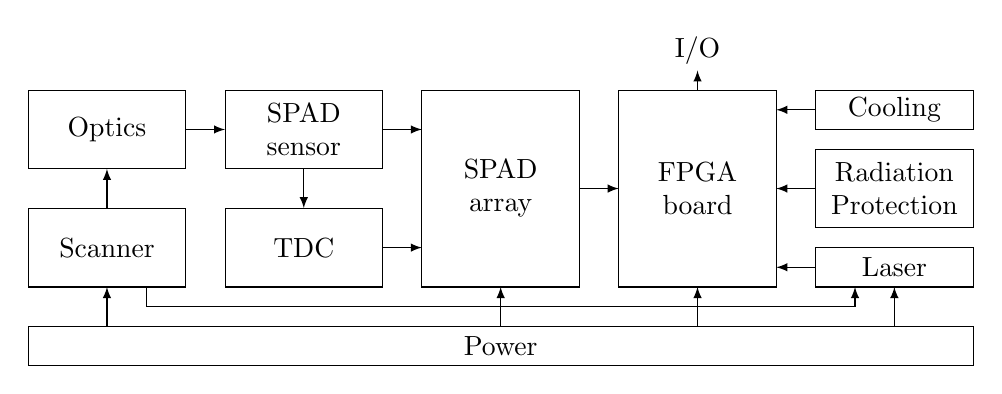
\begin{tikzpicture}[scale=.5]

\draw  (13,2) rectangle (17,1) node[pos=.5, align=center]{Cooling};
\draw  (13,0.5) rectangle (17,-1.5) node[pos=.5, align=center]{Radiation\\Protection};
\draw  (-7,-4) rectangle (17,-5) node[pos=.5, align=center]{Power};
\draw  (13,-2) rectangle (17,-3) node[pos=.5, align=center]{Laser};
\draw  (8,2) rectangle (12,-3) node[pos=.5, align=center]{FPGA\\board};
\draw  (3,2) rectangle (7,-3) node[pos=.5, align=center]{SPAD\\array};
\draw  (-2,2) rectangle (2,0) node[pos=.5, align=center]{SPAD\\sensor};
\draw  (-7,2) rectangle (-3,0) node[pos=.5, align=center]{Optics};
\draw  (-7,-1) rectangle (-3,-3) node[pos=.5, align=center]{Scanner};
\draw  (-2,-1) rectangle (2,-3) node[pos=.5, align=center]{TDC};

\draw [>=latex, ->](0,0) -- (0,-1);
\draw [>=latex, ->](2,-2) -- (3,-2);
\draw [>=latex, ->](13,1.5) -- (12,1.5);
\draw [>=latex, ->](7,-.5) -- (8,-.5);
\draw [>=latex, ->](2,1) -- (3,1);
\draw [>=latex, ->](13,-2.5) -- (12,-2.5);
\draw [>=latex, ->](10,2) -- (10,2.5);
\draw [>=latex, ->](-3,1) -- (-2,1);
\draw [>=latex, ->](13,-.5) -- (12,-.5);
\draw [>=latex, ->](5,-4) -- (5,-3);
\draw [>=latex, ->](10,-4) -- (10,-3);
\draw [>=latex, ->](15,-4) -- (15,-3);
\draw [>=latex, ->](-5,-1) -- (-5,0);
\node at (10,3) {I/O};

\draw [>=latex, ->](-5,-4) -- (-5,-3);
\draw [>=latex, ->](-4,-3) -- (-4,-3.5) -- (14,-3.5) -- (14,-3);

\end{tikzpicture}




    \caption{Schematic overview}
    \label{tkz:schematic_overview}
\end{figure}

~\\
\textbf{Laser}: The laser must send short pulses but powerful pulses at a predefined frequency, to transmit photons that can be detected by the SPAD Sensor. A critical requirement for the laser is the amount of photons it is able to transmit as a function of time, within the budget and technical limitations. \\
\\
\textbf{SPAD Sensor}: The Single Photon Avalanche Diode (SPAD) is responsible for generating a digital pulse when hit by a photon. A circuit build around the SPAD must ensure that the SPAD is quenched as quickly as possible to minimize the deadline. A critical requirement for the SPAD is a small jitter to maximize the accuracy of the sensor.  \\
\\
\textbf{TDC}: The Time Interval to Digital Converter (TDC) is connected to the laser and the SPAD Sensor. The TDC must measure the time difference between the transmission of the laser and the receiving at the SPAD sensor. This measurement requires an accuracy of tens of picoseconds to meet the accuracy requirements.\\
\\
\textbf{Scanner}: The scanner handles the scanning motion that is needed to accumulate the entire picture. Different scanning motions can introduce undesired jitter and heavily influence the amount of SPAD Sensors that are needed on teh SPAD Array. \\
\\
\textbf{SPAD Array}: The SPAD Array integrates the SPAD Sensors on a chip and connects them to the TDCs. The layout of the SPAD Array is closely related to the scanning motion that is used in the scanner.\\
\\
\textbf{Optics}:
The optics must transfer as much of the incoming photons as possible to the sensitive area on the SPAD Sensors. The Optics part also implements a bandpass filter around the target frequency. \\
\\
\textbf{FPGA Board}:
The FPGA Board controls the sensor. It is responsible for accumulating and interpreting the measurements from the TDCs, and controlling the Scanner and Laser. \\
\\
\textbf{Cooling}:
The cooling has to keep the temperature of the FPGA chip under a threshold temperature.\\
\\
\textbf{Radiation Protection}:
The Radiation Protection shields sensitive parts of the sensor from radiation. The most sensitive part of the system is expected to be the FPGA Board, based on experience.\\
\\
\textbf{Power}:
The power block has to supply the scanner, SPAD Array, FPGA Board, and the laser with the required power. The power block has to operate within the specified power budget.











\section{Assumptions} 
\label{ssec:assumptions}
This section will list the assumption that are made throughout the study.\\
\\
\textbf{Reflectivity of surface Europa}: It is assumed that out of all light that hit's Europa, $35\%$ is reflected in a perfectly diffuse manner.\\ 
\\
\textbf{Wavelength laser}: The wavelength of light emitted by the laser is assumed to be $850\,nm$. This wavelength is a typcial choice for Silicon SPAD's. The main reason for this wavelength as opposed to $550\,nm$ is because the that sunlight is less strong in that region, and less background noise will lft after applying a narrow bandpass filter. \\
\\
\textbf{Bandpass filter}:A bandpass filter will be used o filter background noise. This filter is assumed to be a bandpass filter with a center frequency of $850\,nm$ and a FWHM of $10\,nm$.The minimum transmission of the filter is $50\%$. These values are directly taken from the "\textit{850nm, 10nm FWHM, 12.5mm Mounted Diameter}" product made by Edmund Optics and sold for $75\,\$$.\\
\\
\textbf{Jitter of SPAD Sensor}: The jitter of the SPAD Sensor, or Full Width Half Max (FWHM) is assumed to be $100\,ps$. This value is a typical FWHM for state of the art Silicon SPAD's. \\
\\
\textbf{Jitter of TDC}: The jitter of the TDC's is assumed to be insignificant when compared to the jitter of $100\,ps$ caused by the SPAD Sensors. Experience with previous designs show that TDC jitter is generally a very small contributor to overall jitter.\\
\\
\textbf{Resolution of TDC}: The accuracy of the TDC is assumed to be $50\,ps$.\\
\\
\textbf{Sunlight}: It is assumed that the light from the sun that is reflected of Europa is the only signifant contributor to background noise. No other sources of light will be considered. \\
\\
\textbf{Photon Detection Probability}: It is assumed that the PDP of the SPADs is $10\%$.\\
\\
\textbf{Laser light hitting target}: It is assumed that all the light that leaves the laser is hitting the target area on Europa.
\\
\\
\textbf{Laser efficiency}: It is assumed that the laser has an efficiency of $10\%$.




\chapter{Altimetry Mode}\label{sec:altimetry_mode}
The Altimetry Mode is the mode in which only the altitude of the device in relationship to Europa is required. The main challenges for the altimetry mode are acquiring the required resolution, acquiring the required speed, staying within the power budget, and being sufficiently resilient against the accumulated radiation for the entire trip.

The first step will be to create a model of the noise that will be present at Europa. Then the required amount of signal will be calculated, resulting in the required signal power. 

\section{Optics}\label{ssec:optics}
The receiver optics are a good place to start of with, because the optics are not very dependent on results achieved in other areas. The optics have to transport as many desired photons, and as little unwanted photons to the active area on the SPADs as possible. All while having an acceptable depth of field. 

The most basic solution is a single lens with an aperture. The opacity of the lens can be calculated with the absorption of the lens material and f-number of the lens using \cref{eq:basic_opacity}.

\begin{align}\label{eq:basic_opacity}
\text{opacity} = \frac{1-\text{absorption}}{\text{f-number}^2}
\end{align}

 The performance of a possible configuration is shown in \cref{tab:basic_optics}

\begin{table}[H]
\centering
\caption{Performance of basic optics solution}
\label{tab:basic_optics}
\begin{tabular}{|l|r|}\hline
    \textbf{Basic Optics} & \\
    \hline 
    f-number & $2.00\, $ \\
    absorption & $5.00\,\%$ \\
    opacity & $23.75\, \%$ \\
    \hline 
\end{tabular}
\end{table}


\subsection{Improvements}
There are a couple of additions that can improve the performance of the optics. The first and essential one, is the use of a bandpass filter. The transmitted signal will have a very specific bandwidth of $850\,nm$. Using a narrow bandpass filter one can filter out an enormous part of the background noise. The filter will have an opacity of $50\,\%$ for the target wavelength.

The captured photons that hit the lens need to be guided to the active area of the SPADs. If the active area on the chip is very small, one can use microlenses to improve the effectiveness of the optics. A Microlens focuses light on a single SPAD on the chip. Two types of microlenses will be considered: a spherical lens, and a square shaped lens. The presence of microlenses poses a limitation of the main lens. The f-number must be relatively large. A higher f-number means a smaller aperture and therefore more loss of photons. A way of dealing with this problem is to use a second lens instead. An overview of the available options is shown in \cref{tkz:receiver_optics}

\begin{figure}[H]
    \centering


\resizebox{\linewidth*3/4}{!}{
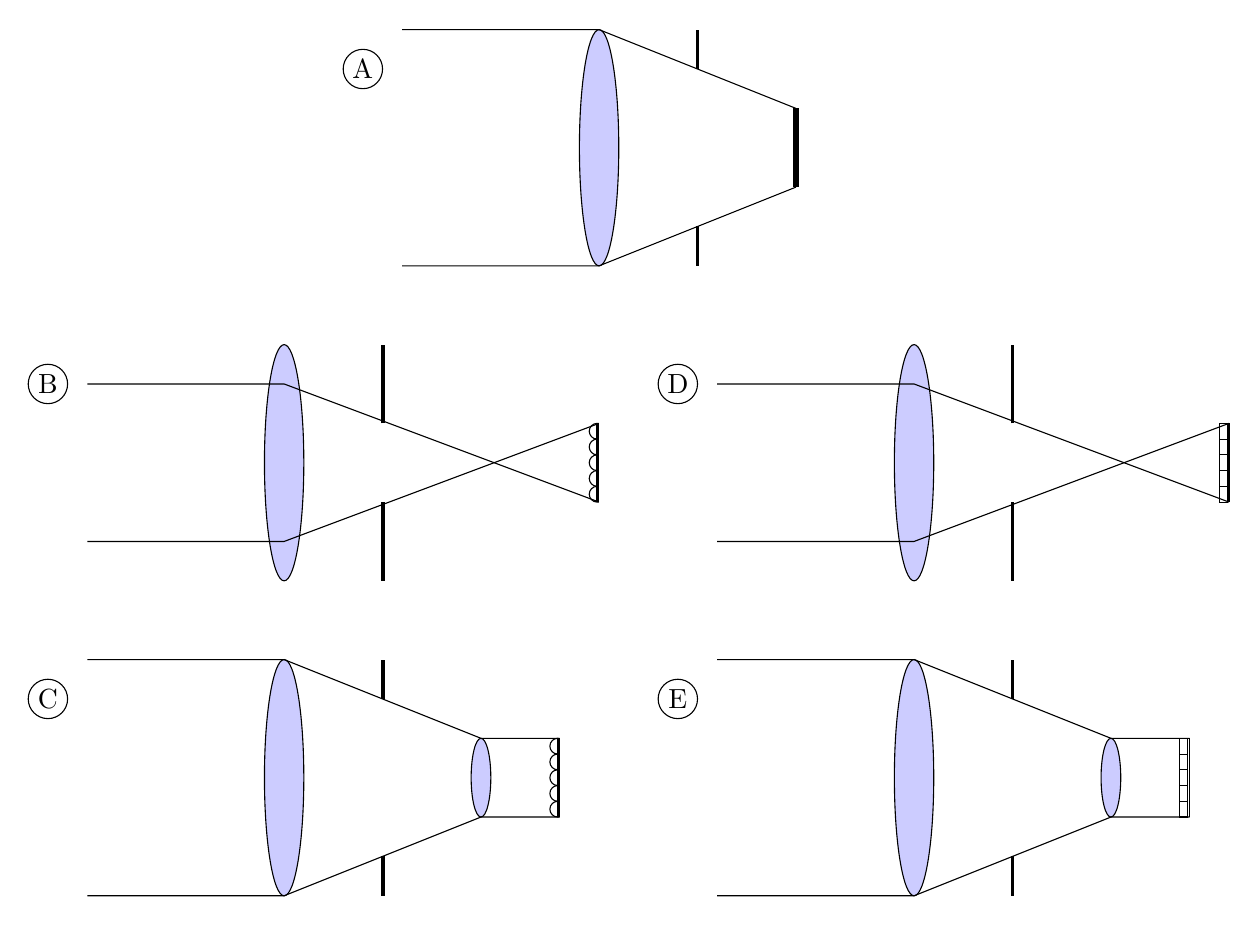
\begin{tikzpicture}[scale=.5]

%%%%%% low F-number, no microlens

%lens
\draw [fill=blue!20] (7,4) ellipse (0.5 and 3);

%diafragma
\draw [line width=.5mm] (9.5,6) -- (9.5,7);
\draw [line width=.5mm] (9.5,1) -- (9.5,2);

%sensitive area
\draw [line width=.7mm] (12,3) -- (12,5);

%light beams
\draw (2,7) to (7,7) to (12,5);
\draw (2,1) to (7,1) to (12,3);

%%%%%%Microlens + high F-number

%lens
\draw [fill=blue!20] (-1,-4) ellipse (0.5 and 3);

%diafragma
\draw [line width=.5mm] (1.5,-3) -- (1.5,-1);
\draw [line width=.5mm] (1.5,-7) -- (1.5,-5);

%sensitive area
\draw [line width=.7mm] (7,-5) -- (7,-3);

%light beams
\draw (-6,-2) to (-1,-2) to (7,-5);
\draw (-6,-6) to (-1,-6) to (7,-3) node (v1) {};


%Microlenses
\draw  (6.95,-3.2) ellipse (.2 and .2);
\draw  (6.95,-3.6) ellipse (.2 and .2);
\draw  (6.95,-4.0) ellipse (.2 and .2);
\draw  (6.95,-4.4) ellipse (.2 and .2);
\draw  (6.95,-4.8) ellipse (.2 and .2);
\fill  (7,-2.8) rectangle (7.4,-5.2) [fill=white];

%%%%%%Microlens + extra lens

%lens
\draw [fill=blue!20] (-1,-12) ellipse (0.5 and 3);

%second lens
\draw [fill=blue!20] (4,-12) ellipse (0.25 and 1);

%diafragma
\draw [line width=.5mm] (1.5,-10) -- (1.5,-9);
\draw [line width=.5mm] (1.5,-15) -- (1.5,-14);

%sensitive area
\draw [line width=.75mm] (6,-13) -- (6,-11);

%light beams
\draw (-6,-9) to (-1,-9) to (4,-11) to (6,-11);
\draw (-6,-15) to (-1,-15) to (4,-13) to (6,-13);


%Microlenses
\draw  (5.95,-11.2) ellipse (.2 and .2);
\draw  (5.95,-11.6) ellipse (.2 and .2);
\draw  (5.95,-12) ellipse (.2 and .2);
\draw  (5.95,-12.4) ellipse (.2 and .2);
\draw  (5.95,-12.8) ellipse (.2 and .2);
\fill  (6,-10.8) rectangle (6.4,-13.2) [fill=white];

%%%%%% Square Microlens + high F-number

%lens
\draw [fill=blue!20] (15,-4) ellipse (0.5 and 3);

%diafragma
\draw [line width=.5mm] (17.5,-3) -- (17.5,-1);
\draw [line width=.5mm] (17.5,-7) -- (17.5,-5);

%sensitive area
\draw  (23,-5) -- (23,-3);

%light beams
\draw (10,-2) to (15,-2) to (23,-5);
\draw (10,-6) to (15,-6) to (23,-3);


%Microlenses
\draw  (22.75,-3) rectangle (22.95,-3.4);
\draw  (22.75,-3.4) rectangle (22.95,-3.8);
\draw  (22.75,-3.8) rectangle (22.95,-4.2);
\draw  (22.75,-4.2) rectangle (22.95,-4.6);
\draw  (22.75,-4.6) rectangle (22.95,-5);


%%%%%% Square Microlens + extra lens

%lens
\draw [fill=blue!20] (15,-12) ellipse (0.5 and 3);

%second lens
\draw [fill=blue!20] (20,-12) ellipse (0.25 and 1);

%diafragma
\draw [line width=.5mm] (17.5,-10) -- (17.5,-9);
\draw [line width=.5mm] (17.5,-15) -- (17.5,-14);

%sensitive area
\draw  (22,-13) -- (22,-11);

%light beams
\draw (10,-9) to (15,-9) to (20,-11) to (22,-11);
\draw (10,-15) to (15,-15) to (20,-13) to (22,-13);


%Microlenses
\draw  (21.75,-11) rectangle (21.95,-11.4);
\draw  (21.75,-11.4) rectangle (21.95,-11.8);
\draw  (21.75,-11.8) rectangle (21.95,-12.2);
\draw  (21.75,-12.2) rectangle (21.95,-12.6);
\draw  (21.75,-12.6) rectangle (21.95,-13);



\draw  (1,6) ellipse (.5 and .5) node[]{A};
\draw  (-7,-2) ellipse (.5 and .5) node[]{B};
\draw  (-7,-10) ellipse (.5 and .5) node[]{C};
\draw  (9,-2) ellipse (.5 and .5) node[]{D};
\draw  (9,-10) ellipse (.5 and .5) node[]{E};


\end{tikzpicture}
}

    \caption{Overview of possible receiver optics implementations}
    \label{tkz:receiver_optics}
\end{figure}

\begin{align}
\text{opacity} = (1-\text{absorption}_1)(1-\text{absorption}_2)\cdot\text{opacity filter}\cdot \frac{X}{\text{f-number}^2}
\end{align}
Where $X$ is the active area on the chip. A comparison between the different options is shown in \cref{tab:receiver_optics}

\begin{table}[H]
\centering
\caption{comparison of different optics solutions}
\label{tab:receiver_optics}
\begin{tabular}{|l|lllll|}\hline
\textbf{Type}                & \textbf{A}        & \textbf{B}        & \textbf{C}        & \textbf{D}        & \textbf{E}        \\ \hline
absorption $1^{st}$ lens & 0.05     & 0.05     & 0.05     & 0.05     & 0.05     \\
f-number                 & 2        & 8        & 2        & 8        & 2        \\
absorption $2^{nd}$ lens & 0        & 0        & 0.05     & 0        & 0.05     \\
active area on chip      & 0.05     & 0.55     & 0.55     & 0.65     & 0.65     \\ \hline
effective opacity            & 0.011875 & 0.008164 & 0.124094 & 0.009648 & 0.146656 \\ \hline
\end{tabular}
\end{table}

The comparison in \cref{tab:receiver_optics} shows some good alternatives to the basic lens, if there is a need for it due to a small active area on the chip. However, most of the future calculations will focus on the basic model A.


\section{Noise caused by the sun}\label{ssec:background_noise}
The sun is the most dominant source of unwanted photons at Europa. This section will investigate how much energy is hitting the surface of Europa. 

To calculate that the sun will be modelled as an ideal black body. The spectral irradiance of the sun can be calculated using \cref{eq:spectral_irradiance}.
\begin{align}\label{eq:spectral_irradiance}
I_\lambda(\lambda,T) = \frac{2hc^2}{\lambda^5}\frac{1}{e^{\frac{hc}{\lambda kT}}-1}
\end{align}
where $I_\lambda(v,t)$ is spectral irradiance with unit $W/m^3$. \\
$h$ is the planck constant\\
$c$ is the speed of light in vacuum \\
$k$ is the Boltzman constant \\
$\lambda$ is the wavelength of the electromagnetic radiation\\
$T$ is the absolute temperature of the body\\



The spectral irradiance of the sun is calculated in \cref{tab:sun_irradiation}.

\begin{table}[H]
\centering
\caption{Calculation of sun irradiation}
\label{tab:sun_irradiation}
\begin{tabular}{|l|l|}\hline
    \textbf{Sun irradiation} & \\
    \hline 
    $h$ & $663.00\cdot10^{-36}\,Js$ \\
    $c$ & $300.00\cdot10^6\,m/s$ \\
    $k$ & $13.80\cdot10^{-24}\,j/K$ \\
    $\lambda$ & $850.00\,n m$ \\
    $I_\lambda$ & $15.11\cdot10^{12}\,W/m^3$ \\
    \hline 
\end{tabular}
\end{table}


The next step is to calculate the power emitted by the sun in the specified bandwidth, at the location of Europa. The specified bandwidth is in this case the assumed bandpass filter used on the lens. The emitted power is calculated by modelling the sun as a point source, and then spreading that power over a sphere with a radius equal to the distance between the sun and Europa, as is done in \cref{eq:point_source}.

\begin{align}\label{eq:point_source}
    P_{sun} = I_{\text{sun}} B_\lambda S \frac{r_{\text{sun}}^2}{r_{\text{europa}}^2}
\end{align}
where $I_{\text{sun}}$ is the spectral irradiance of the sun at the center frequency of the filter, $B_\lambda$ is the bandwidth of the filter in meters, $S$ the surface area of the target area on Europa, $r_{\text{sun}}$ the of radius of the sun, and $r_{\text{europa}}$ the distance between Europa and the sun. The effective radiance of the background noise at Europa is calculated in \cref{tab:background_power} using \cref{eq:point_source}.

\begin{table}[H]
\centering
\caption{Calculation of background power on target area on Europa}
\label{tab:background_power}
\begin{tabular}{|l|r|}\hline
    \textbf{Background power} & \\
    \hline 
    $I_\lambda$ & $15.11\cdot10^{12}\,W/M^3$ \\
    $B_\lambda$ & $10.00\,n m$ \\
    Surface area & $10000.00\, m^2$ \\
    $r_{sun}$ & $695.70\,\,km$ \\
    $r_{europa}$ & $800.00\cdot10^3\,km$ \\
    $P_B$ & $1.14\,k W$ \\
    \hline 
\end{tabular}
\end{table}


The next step is to calculate the percentage of energy that hits the device when hovering over Europa. The focal length and aperture ofthe lens will be configured in such a way that the target surface on Europa fills the entire view at the maximum altitude of the Hazard Detection Mode, so that altitude will be chosen to calculate the received noise power. The amount of power received at the lens of the device can be calculated using \cref{eq:power_lens}.

\begin{align}\label{eq:power_lens}
P'_B = \frac{P_B\cdot R_{Europa}\cdot D_l\cdot \text{opacity}}{2r^2}
\end{align}
where $P'_B$ is the power hitting the lens, \\
$P_B$ the noise power on the target area of Europa,\\
$R_{Europa}$ the reflectivity of Europa,\\
$D_l$ the diameter of the lens,\\
opacity the opacity of the lens,\\
and $r$ the altitude of the device. The calculations are performed in \cref{tab:effective_noise_power}.

\begin{table}[H]
\centering
\caption{Pulse frequency for both modes of operation}
\label{tab:effective_noise_power}
\begin{tabular}{|l|r|}\hline
    \textbf{effective noise power} & \\
    \hline 
    $P_B$ & $1.89\,m W$ \\
    $r$ & $500.00\, m$ \\
    $R_{europa}$ & $35.00\, \%$ \\
    Diameter lens $(D_l)$ & $50.00\,m m$ \\
    opacity filter $(L_f)$ & $50.00\, \%$ \\
    opacity optics $(L_l)$ & $14.60\, \%$ \\
    $P_B2$ & $4.82\,p W$ \\
    \hline 
\end{tabular}
\end{table}


Finally the power needs to be converted to number of photons. To calculate how many photons bounce from the surface of Europa and actually hit the light. To calculate the amount of photons one needs to know the amount of energy per photon. This can be calculated using \cref{eq:e_photon}. The calculation is performed in \cref{tab:energy_of_photon}.

\begin{align}\label{eq:e_photon}
E_{photon} = \frac{hc}{\lambda}
\end{align}

\begin{table}[H]
\centering
\caption{Pulse frequency for both modes of operation}
\label{tab:energy_of_photon}
\begin{tabular}{|l|r|}\hline
    \textbf{energy of photon} & \\
    \hline 
    $h$ & $663.00\cdot10^{-36}\,Js$ \\
    $c$ & $300.00\cdot10^6\,m/s$ \\
    $\lambda$ & $850.00\,n m$ \\
    $E_{photon}$ & $234.00\cdot10^{-21}\,J$ \\
    \hline 
\end{tabular}
\end{table}
 

The amout of photons per second can then be calculated using \cref{eq:PPS}. The calculation is shown in

\begin{align}\label{eq:PPS}
\text{photon}/s = \frac{P}{E_{photon}}
\end{align}

\begin{table}[H]
\centering
\caption{Pulse frequency for both modes of operation}
\label{tab:photons_hitting_SPADs}
\begin{tabular}{|l|r|}\hline
    \textbf{photons hitting SPADs} & \\
    \hline 
    $P'_B$ & $7.76\cdot10^{-6}\,W$ \\
    $E_{photon}$ & $2.34\cdot10^{-19}\,J$ \\
    photons at SPADs & $3.31\cdot10^{13}\,\text{photon}/s$ \\
    \hline 
\end{tabular}
\end{table}













% \section{Scanning motion}\label{ssec:scanning_motion}
In \cref{ssec:SPADs}, it was concluded that a SPAD array with one SPAD per pixel is not feasible. Therefore a scanning motion is required. Possible scanning motions for different SPAD array configurations are shown in \cref{tkz:scanning_motions}. Note that the $2048\times1$ motion is in essence a special case of the $2048\times N$ motion, where exactly one row of pixels is observed at a time. The $M\times N$, with $M<2048$ and $N<2048$ needs a scanning motion in both $x$ and $y$ direction. This makes the scanning motion very complicated and unreliable. Therefore only the family of solutions with $2048\times N$ with $N<2048$ will be considered.


\begin{figure}[H]
    \centering
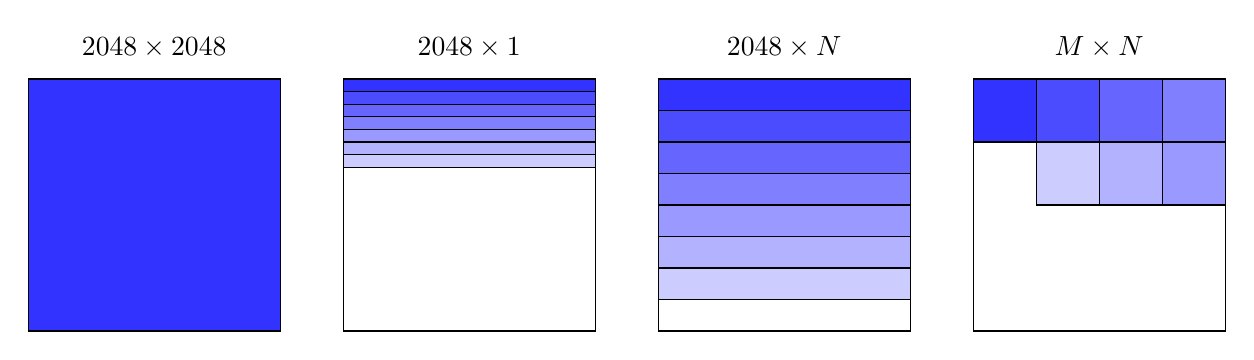
\begin{tikzpicture}[scale=.8]
\draw  (-3,4) rectangle (1,0);
\draw [fill=blue!80] (-3,4) rectangle (1,3.8);
\draw [fill=blue!70] (-3,3.8) rectangle (1,3.6);
\draw [fill=blue!60] (-3,3.6) rectangle (1,3.4);
\draw [fill=blue!50] (-3,3.4) rectangle (1,3.2);
\draw [fill=blue!40] (-3,3.2) rectangle (1,3);
\draw [fill=blue!30] (-3,3) rectangle (1,2.8);
\draw [fill=blue!20] (-3,2.8) rectangle (1,2.6);


\draw  (2,4) rectangle (6,0);
\draw [fill=blue!80] (2,4) rectangle (6,3.5);
\draw [fill=blue!70] (2,3.5) rectangle (6,3);
\draw [fill=blue!60] (2,3) rectangle (6,2.5);
\draw [fill=blue!50] (2,2.5) rectangle (6,2);
\draw [fill=blue!40] (2,2) rectangle (6,1.5);
\draw [fill=blue!30] (2,1.5) rectangle (6,1);
\draw [fill=blue!20] (2,1) rectangle (6,0.5);


\draw  (7,4) rectangle (11,0);
\draw [fill=blue!80] (7,4) rectangle (8,3);
\draw [fill=blue!70] (8,4) rectangle (9,3);
\draw [fill=blue!60] (9,4) rectangle (10,3);
\draw [fill=blue!50] (10,4) rectangle (11,3);
\draw [fill=blue!40] (10,3) rectangle (11,2);
\draw [fill=blue!30] (9,3) rectangle (10,2);
\draw [fill=blue!20] (8,3) rectangle (9,2);

\node at (-6,4.5) {$2048\times2048$};
\node at (-1,4.5) {$2048\times1$};
\node at (4,4.5) {$2048\times N$};
\node at (9,4.5) {$M\times N$};

\draw [fill=blue!80] (-8,4) rectangle (-4,0);
\end{tikzpicture}
    \caption{Different types of scanning motions}
    \label{tkz:scanning_motions}
\end{figure}

\section{Detected photon characterisation}\label{ssec:HDM_detected_photon_characterisation}
This section is similar to \cref{ssec:detected_photon_characterisation}, but recalculates parts that are different for the HDM mode. First of all, the results of all the SPAD measurements are no longer bundled together, but interpreted seperately. Also the device is a lot closer to Europa with an altitude of at most $500\,m$ which causes the laser to be me more effective when compared to the noise. The new values to work with are shown in \cref{tab:photons_per_SPAD}. Note that the $PPS_S$ is the amount of photons per Watt of optical transmitted energy.


\begin{table}[H]
\centering
\caption{Amount of backgroun (B), dark count (N), and signal (S) photons that hit a single SPAD per second}
\label{tab:photons_per_SPAD}
\begin{tabular}{|l|r|}\hline
    \textbf{photons per SPAD} & \\
    \hline 
    $PPS_B$ & $3.54\cdot10^{8}\,\text{photon}/s$ \\
    $PPS_N$ & $2.00\,k \text{photon}/s$ \\
    $PPS_S$ & $9.39\,k \text{photon}/s$ \\
    \hline 
\end{tabular}
\end{table}


Another important changed property, is that the maximum time of flight $t_{round}=3.33\,\mu s$. This directly means that per measurement, less noise is received. However, the expected amount of noise per bin remains the same. The new $\mu_n=\frac{3.33\cdot10^{-6}}{2}=1.67\,\mu s$, and the new $\sigma_n=\frac{3.33\cdot10^{-6}}{\sqrt{12}}=304\,ns$. 

\section{Sampling Method}\label{ssec:sampling_method}
The sampling method used has a massive impact on the performance of the system. This section investigates the options that can be chosen from.

The time that the sensor should listen to a response is determined by the maximum round trip time of a photon, and can be calculated using \cref{eq:roundtrip}.

\begin{align}\label{eq:roundtrip}
t_{round} = \frac{2r}{c}
\end{align}
where $c\approx 3\cdot10^8$ is the speed of light, and $r$ the altitude of the sensor. 

The next step is to calculate the relationship between oberved number of good and bad photons for a given listening period, and the resulting standard deviation of the measurement. To calculate the standard deviation of the sum of multiple random variables that are statistically independent, one can use \cref{eq:variance_weighted_sum}

\begin{align}\label{eq:variance_weighted_sum}
\newcommand{\Var}{\mathrm{Var}}
 	\Var[aX+bY+cZ] = a^2\Var[X]+b^2\Var[Y]+c^2\Var[Z]
\end{align}

Because the DCR and sunlight photons have the same uniform distribution they are taken from the same uniform random variable $N$, where $n$ is the amount of detected sunlight and dark photons, $\mu_n = \frac{1}{2}t_{round}$, and $\sigma_n=\frac{1}{\sqrt{12}}t_{round}$. The signal photons are taken from the random variable $S$, where $s$ is the amount of detected signal photons, $\mu_s= ToF$, and $\sigma_s=42.5\,ps$. The resulting mean $\mu_{tot}$ can be calculated using \cref{eq:mu_tot}. The error with the desired $\mu$ can be calculated using \cref{eq:mu_error}.

\begin{align}
\mu_{tot}&=\frac{1}{s+n}\Big(\sum_{k=1}^s\mu_s+\sum_{l=1}^n\mu_n  \Big)\\
&= \frac{s\cdot Tof}{s+n}+\frac{n\cdot \frac{1}{2}t_{round}}{s+n} \label{eq:mu_tot} 
\end{align}

\begin{align}
\mu_{\text{error}} &= |ToF-\mu_{tot}|\\
&= \Big|\frac{n(ToF-\frac{1}{2}t_{round})}{s+n}\Big|\label{eq:mu_error}
\end{align}

The resulting standard deviation $\sigma_{tot}$ can be calculated using \cref{eq:sigma_tot}.

\begin{align}
\text{Var}_{tot} &= \text{Var}\Big[\frac{1}{s+n}\Big(\sum_{k=1}^s\text{Var}_s+\sum_{l=1}^n\text{Var}_n\Big)\Big]\\
&= \frac{1}{(s+n)^2}(s\sigma_s^2+n\sigma_n^2)\\
\sigma_{tot} &= \sqrt{\text{Var}_{tot}}\\
&= \frac{\sqrt{s\sigma_s^2+n\sigma_n^2}}{s+n} \label{eq:sigma_tot}
%&= \frac{\sqrt{s\cdot(42.5\cdot10^{-12})^2+n\cdot(\frac{1}{\sqrt{12}}t_{round})^2}}{s+n} \\
%&= \frac{\sqrt{s\cdot1.8063\cdot10^{-21}+\frac{n}{12}t_{round}}}{s+n} \label{eq:sigma_tot}
\end{align}

Using \cref{eq:sigma_tot}, one can calculate the relationship between the amount of signal photons needed for a given amount of noise photons. For the long distance a $t_{round}=53.3\,\mu s$ is used. Using \cref{eq:s_vs_n} the realtionship between the number of noise photons and required signal photons is shown in \cref{fig:altimetry_s_vs_n}. Note that the amount of required signal photons first rises quickly, then slowly, and finally even drops. The reason for this trend is that increasing the number of random samples also decreases the standard deviation by itself. \Cref{fig:altimetry_s_vs_n_small} shows the same relationship for a smaller number of noise photons. 
\begin{align}
\sigma_{tot} &= \frac{\sqrt{s\sigma_s^2+n\sigma_n^2}}{s+n} \\
s &= \frac{\sigma_s^2+\sqrt{\sigma_s^4-4\sigma_s^2\sigma_{tot}^2n+4\sigma_n^2\sigma_{tot}^2n}-2\sigma_{tot}^2n}{2\sigma_{tot}^2}\label{eq:s_vs_n}
\end{align} 

\begin{figure}[h]
\centering
	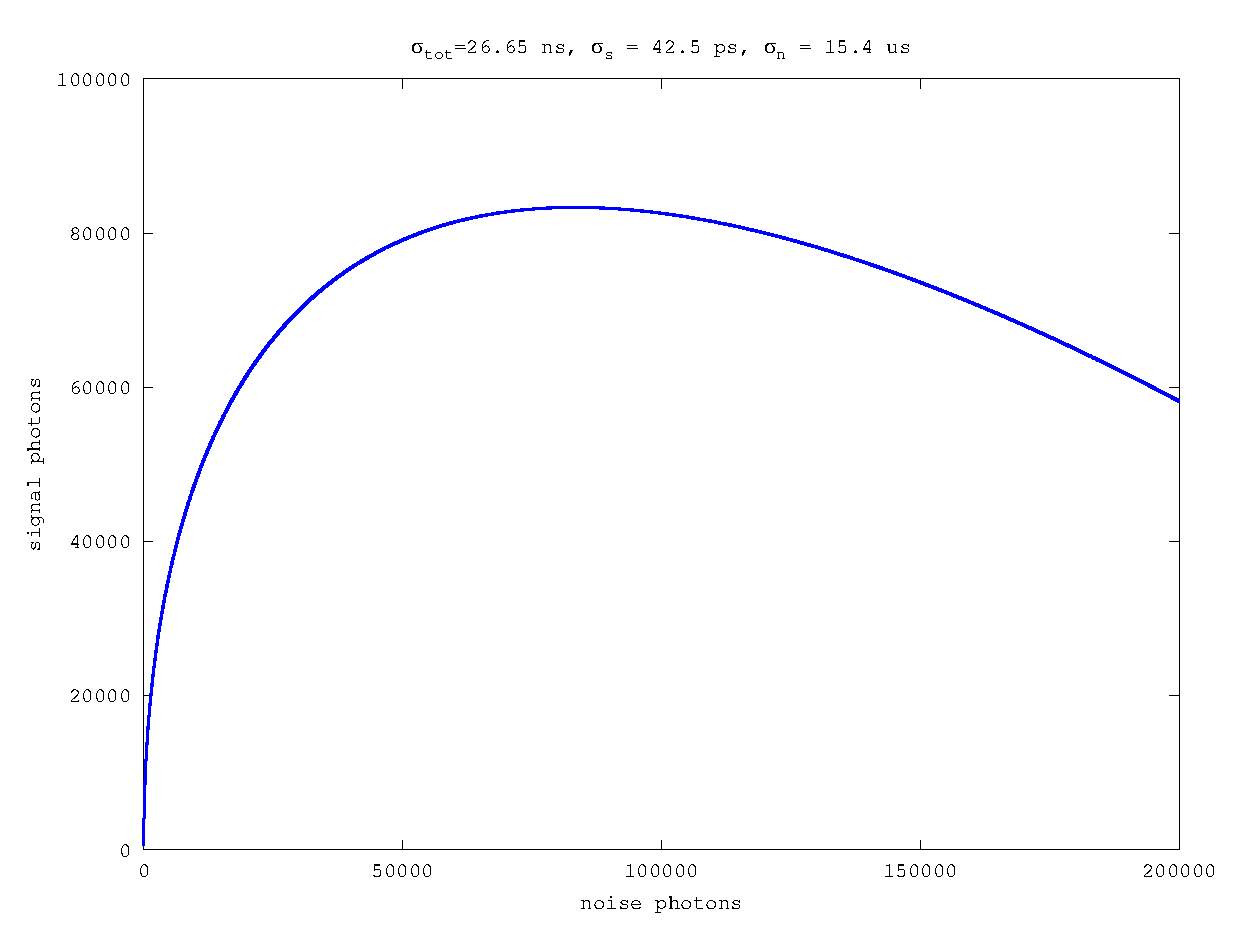
\includegraphics[width=0.8\linewidth]{fig/altimetry_s_vs_n.eps}
\caption{Relationship between number of signal and noise photons to get the required resolution}
\label{fig:altimetry_s_vs_n}
\end{figure}

\begin{figure}[h]
\centering
	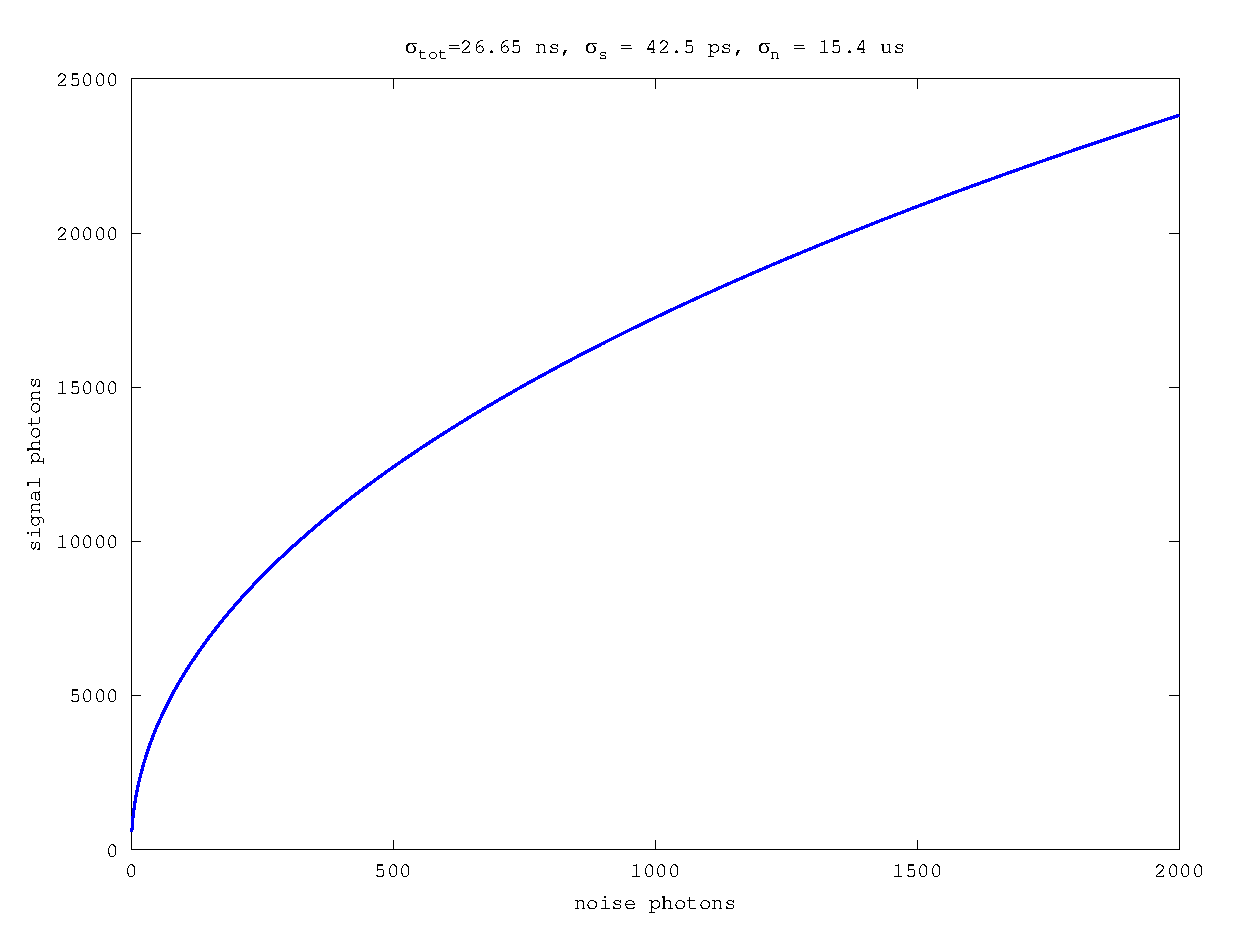
\includegraphics[width=0.8\linewidth]{fig/altimetry_s_vs_n_small.eps}
\caption{Relationship between number of signal and noise photons to get the required resolution}
\label{fig:altimetry_s_vs_n_small}
\end{figure}

% ------------- threshold
\subsection{Energy Threshold}\label{sssec:energy_threshold}
An energy threshold can be a very powerful way to improve signal to noise ratio. The signal photons all arrive with a $FWHM = 100\,ps$, while the noise photons are spread out over $53.3\,\mu s$. An energy threshold is a perfect way to take advantage of this. When the phoons are divided over bins, the expected number of bins can be modelled as Poission process. Using this the efficiency of the energy threshold can be perfomed which is shown in \cref{fig:threshold_efficiency}, where the opacity is 1 if all photons pass through the threshold, and 0 if no photons pass through the threshold. It is important to notice that a certain threshold has no effect at all if the expected number of photons is sufficiently high. The threshold is most effective when the opcity for the signal photons is close to 1, and the opacity for noise photons close to 0. To apply a threshold however, one needs to assemble a historgram of all the detections. The feasability of such a histogram will be investigated later, but for now both a system with and without an energy threshold are considered.  

\begin{figure}[H]
\centering
	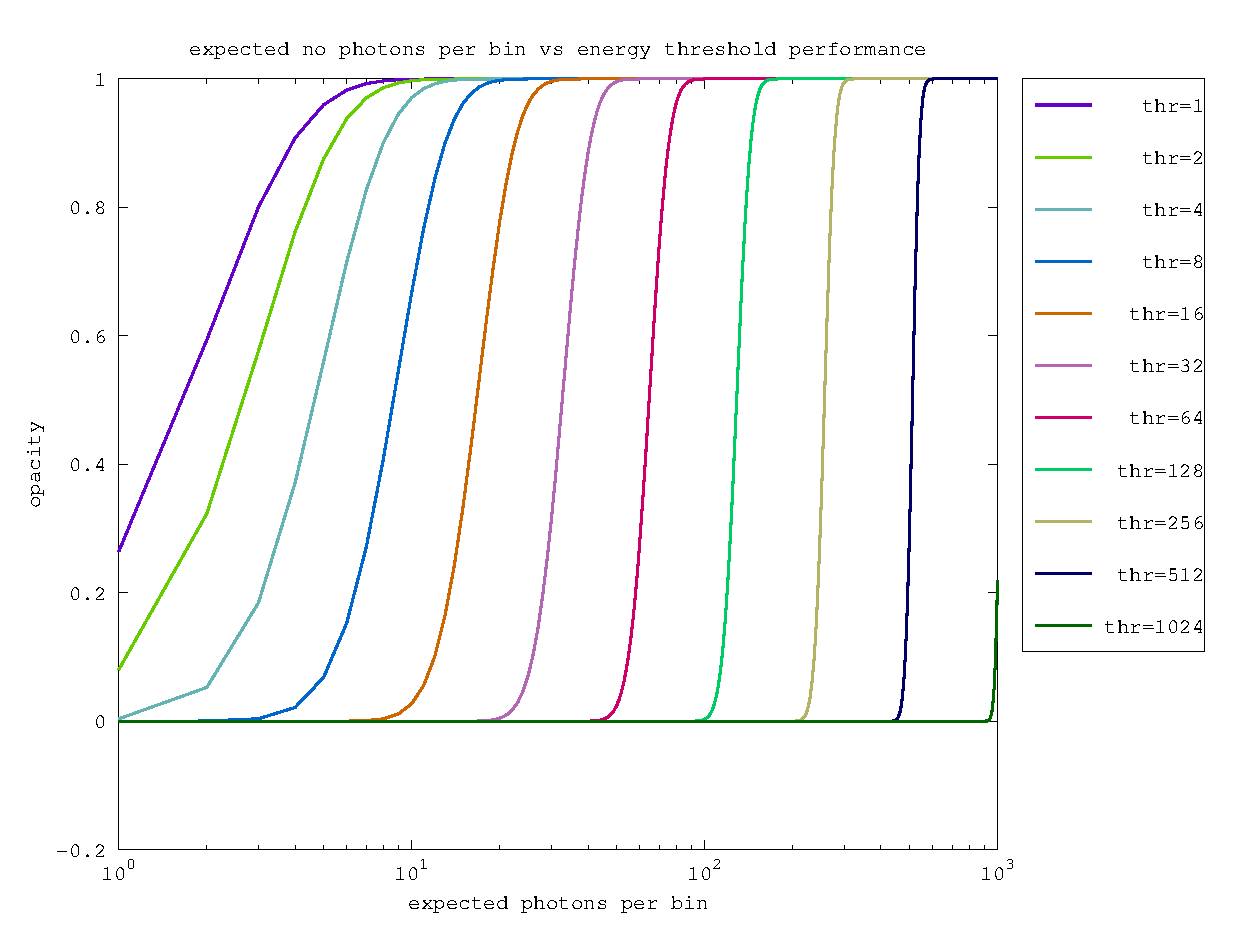
\includegraphics[width=0.8\linewidth]{fig/threshold_efficiency.eps}
\caption{Expected number of photons per bin versus the opacity of the threshold, where opacity=1 means all photons pass through the threshold, and opacity=0 means no photons pass through the threshold}
\label{fig:threshold_efficiency}
\end{figure}


%-----------------------------------------
% \subsubsection{Two frequency sampling}

% The maximum pulse frequency can then be calculated using \cref{eq:pulse_f}

% \begin{align}\label{eq:pulse_f}
% f_{pulse} = \frac{1}{t_{round}} = \frac{c}{2r}
% \end{align}



% The maximum altitude are different for the Altimetry and Hazard Detection mode. The maximum pulse frequency of both modes is shown in \cref{tab:pulse_frequency}.

% %\begin{table}[H]
\centering
\caption{Pulse frequency for both modes}
\label{tab:pulse_frequency}
\begin{tabular}{|l|ll|}
\hline
\textbf{Pulse Frequency}      &      Altimetry & Hazard Detection    \\ \hline
Maximum altitude  &  $8\,km$ & $500\, m$\\ 
Roundtrip time      &  $53.3\,\mu s$ & $3.33\,\mu s$ \\
Pulse frequency     & $18.75\,kHz$    & $300\,kHz$  \\ \hline
\end{tabular}
\end{table}


% In order to increase the frequency, it is intersting to see what happens if the frequency is increased. The TDC measures the time between the last outgoing pulse and the incomming pulse. This means that the performed measurement $t_{TDC}$ can be calculated using \cref{eq:t_TDC_ToF}.

% \begin{align}\label{eq:t_TDC_ToF}
% 	t_{TDC} &=ToF \mod T_{pulse}\\	
% 	ToF &= t_{TDC}+k\cdot T_{pulse} & k \in \mathbb{N}\label{eq:ToF_t_TDC}
% \end{align}

%  where $t_{TDC}$ is the measurement of the TDC, $ToF$ the time of flight, and $T_{pulse}$ the time period of the laser pulses. The returned answer is related to $ToF$ as shown in \cref{eq:ToF_t_TDC}. The precision of the measurement is maintained,  but on a larger scale the information is lost. \\
%  \\
% To solve this problem one can make measurements in two different frequencies. The idea is also applied in TDCs (Name of technique?), where two ring oscillators with different frequencies are used to amplify the range of the TDC. A similar idea can be applied here, but instead of using two oscillators, the time is devided in half, and in the first half the laser sends pulses in frequency $f_1$, and in the second half pulses with frequncy $f_2$. These two different measurements can first be used to determine the large scale ToF, and then the measurements can be combined to get a high accuracy to accompany that.\\
% \\
% As a proof of concept. This idea is applied to the Altimetry Mode. It is assumed that a difference of $5\,ns$ between $\lambda_1$ and $\lambda_2$ is sufficient. Now using a maximum $ToF$ one can calculate that optimal two frequencies, such that $f1_>f_2$ and $f_2$ as high as possible. 

% \begin{align}
%  	\frac{50\mu}{5n} &= 10660\\ 
%  	\sqrt{\frac{50\mu}{5n}} &\approx 103
%  \end{align} 
%  Now two coprime numbers in $\mathbb{N}$ around 103 are 103 and 104. The resulting frequencies are
%  \begin{align}
%  	T_1 &= 103\cdot5n = 515n\\
%  	T_2 &= 104\cdot5n = 520n\\
%  	f_1 &= \frac{1}{T_1} = 1.9417\,MHz\\
%  	f_2 &= \frac{1}{T_1} = 1.9231\,MHz\\
%  \end{align}
% The pulse frequency increases by a factor 100. A matlab plot of the resulting system is shown in \cref{fig:frequency_hopping}, where the measurement values of the TDC are plotted against the $ToF$.


% \begin{figure}[h]
%     \centering
%     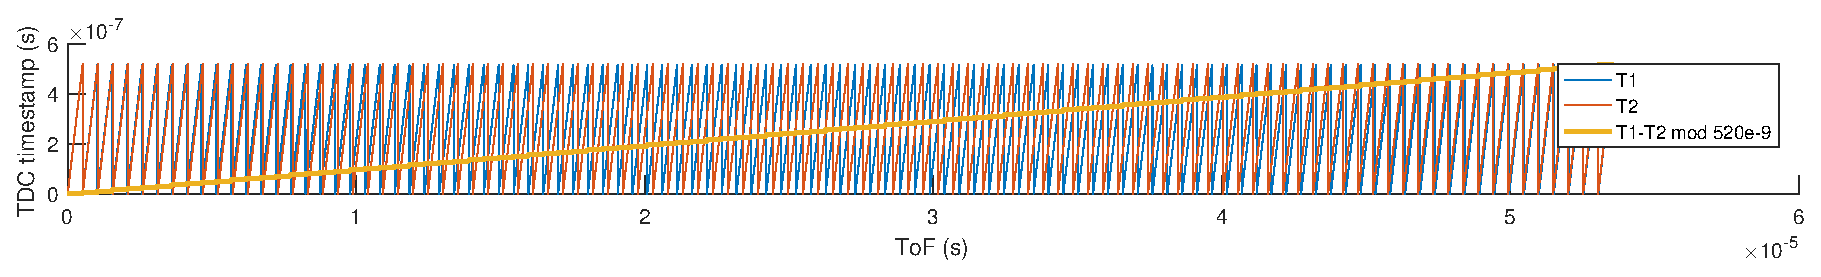
\includegraphics[width=\textwidth]{fig/frequency_hopping.eps}
%     \caption{Matlab plot of TDC measurements vs ToF}
%     \label{fig:frequency_hopping}
% \end{figure}

% The $ToF$ can be calculated using \cref{eq:ToF}.

% \begin{align}
% 	t_{1-2} &= (t_1-t_2)\mod T_2\\
% 	ToF &= \frac{t_{1-2}}{T_2-T_1}T_1+\frac{t_1+t_2-t_{1-2}}{2}\label{eq:ToF}
% \end{align}
% where $t_1$ and $t_2$ are the timestamp measurements for $f_1$ and $f_2$ respectively. $t_{1-2}$ is the modulus of the time difference between $t_1$ and $t_2$.

\subsection{Resolution} 
\label{ssec:resolution}
The requirement for the altimetry mode changes based on the height. The target is a resolution of at least $0.1\,\%$. To ensure that this requirement is met, both the largest altitude of $8\,km$, and the smallest altitude of $500\,m$ will be investigated.

The minimum resolution for the largest and shortest altitude are $8\,m$ and $0.5\,m$ respectively. The maximum allowable FWHM can be calculated using \cref{eq:max_FWHM}.
 Using \cref{eq:FWHM_sigma} the maximum standard deviation can be calculated. The calculations are performed

\begin{align}\label{eq:max_FWHM}
FWHM_{max} = \frac{2x}{c}
\end{align}

\begin{table}[H]
\centering
\caption{Required standard deviation to meet the system requirements}
\label{tab:AM_requirements}
\begin{tabular}{|l|rr|}\hline
    \textbf{AM requirements} & short & long \\
    \hline 
    altitude & $500\,m$ & $8\,km$ \\
    resolution & $50\,cm$ & $8\,m$ \\
    FWHM & $3.33\,n s$ & $53.33\,n s$ \\
    $\sigma$ & $1.42\,n s$ & $22.65\,n s$ \\
    \hline 
\end{tabular}
\end{table}








%\subsubsection{standard deviation shortcut}
To calculate the standard deviation of the sum of multiple random variables that are independent and uncorrelated, one can use \cref{eq:variance_weighted_sum}


\begin{align}\label{eq:variance_weighted_sum}
\newcommand{\Var}{\mathrm{Var}}
 	\Var[aX+bY+cZ] = a^2\Var[X]+b^2\Var[Y]+c^2\Var[Z]
\end{align}




Next consider a situation where there are two random variable distributions. The first distribution is $S$, which is a normal distribution with $\mu_s=ToF$, where $ToF \in \{0, 50\mu\}$, and $\sigma_s=100p$. The second distribution is $N$, which is a uniform distribution with $\mu_n=\frac{50\mu}{2}$ and $\sigma_n=\frac{50\mu}{\sqrt{12}}$.

\begin{align}
	\mu_{mean} &= \frac{1}{110}\Big(\sum_{k=1}^{100}\mu_s+\sum_{l=1}^{10}\mu_n\Big)\\
			   &= \frac{100ToF+10*25\mu}{110}\\
			   &= \frac{10}{11}ToF+227.3n
\end{align}


\begin{align}
	\mathrm{Var}_{mean} &= \mathrm{Var}\Big[\frac{1}{110}\Big(\sum_{k=1}^{100}S_k+\sum_{l=1}^{10}N_l\Big)\Big]\\ 
	 &= \frac{1}{110^2}\Big(\sum_{k=1}^{100}\mathrm{Var}[S]+\sum_{l=1}^{10}\mathrm{Var}[N]\Big)\\
	&= \frac{1}{110^2}(100\sigma_s^2+10\sigma_n^2)\\
	&= \frac{10^{-18}+2.0833\cdot10^{-9}}{110^2}\\
	&= 1.7218\cdot10^{-13}\\
	\sigma_{mean} &= \sqrt{\mathrm{Var}_{mean}}\\
				  &= 414.94n
\end{align}



% Now we grab 100 samples out of $S$ and 10 out of $N$. First, the $\sigma$ and $\mu$ of the average of the 100 samples of $S$ is calculated.

% \begin{align}
% 	\mu_{s,mean} &= \frac{1}{100}\sum_{k=1}^{100}\mu_s\\
% 			     &= ToF
% \end{align}

% \begin{align}
% 	\mathrm{Var}[\frac{1}{100}\sum_{k=1}^{100}S_k] &= \frac{1}{100^2}\sum_{k=1}^{100} \mathrm{Var}[S_k]\\
% 						  &= \frac{\mathrm{Var}[S]}{100}\\
% 	\sigma_{s,mean} &= \frac{\sigma_s}{\sqrt{100}}\\
% 					&= 10p
% \end{align}

% Next the average of 10 samples of $N$ is calculated.

% \begin{align}
% 	\mu_{n,mean} &= \frac{1}{10}\sum_{k=1}^{10}\mu_n\\
% 			     &= 25\mu
% \end{align}

% \begin{align}
% 	\mathrm{Var}[\frac{1}{10}\sum_{k=1}^{10}] &= \frac{1}{10^2}\sum_{k=1}^{10} \mathrm{Var}[N_k]\\
% 						  &= \frac{\mathrm{Var}[N]}{10}\\
% 	\sigma_{s,mean} &= \frac{\sigma_n}{\sqrt{10}}\\
% 					&= \frac{50\mu}{\sqrt{120}}
% 					&\approx 4.5644\mu
% \end{align}

% Next the two resulting functions are combined

\chapter{Hazard Detection Mode}\label{sec:hazard_detection_mode}
The Hazard Detection Mode is the mode of operation that operates closer to Europa than the Altimetry Mode. The main difference and challenge is however, is that this time a detailed heightmap must be formed. Therefore, for the Hazard Detection Mode, the layout of the SPADs and the scanning method are essential in determining the feasability of the device. 


\subsection{Types of SPADs}\label{ssec:SPADs}
In Hazard Detection Mode, individual SPADs will have the responsibility of measuring their part in the target. Therefore it is important to first investigate what type of SPAD is best suited for the device. As mentioned in \cref{ssec:optics}, SPADs can have microlenses. Two types are considered: conventional spherical lenses, and rectangular lenses. Spherical lenses typically achieve an effective active area of approximately $55\,\%$, while rectangular lenses typically get an effective active area of appeoximately $65\,\%$. The active area can also be shaped in different sizes, and a circular and rectangular shape are considered here. An overview of the different options is shown in \cref{tkz:SPAD_types}.


\begin{figure}[H]
    \centering

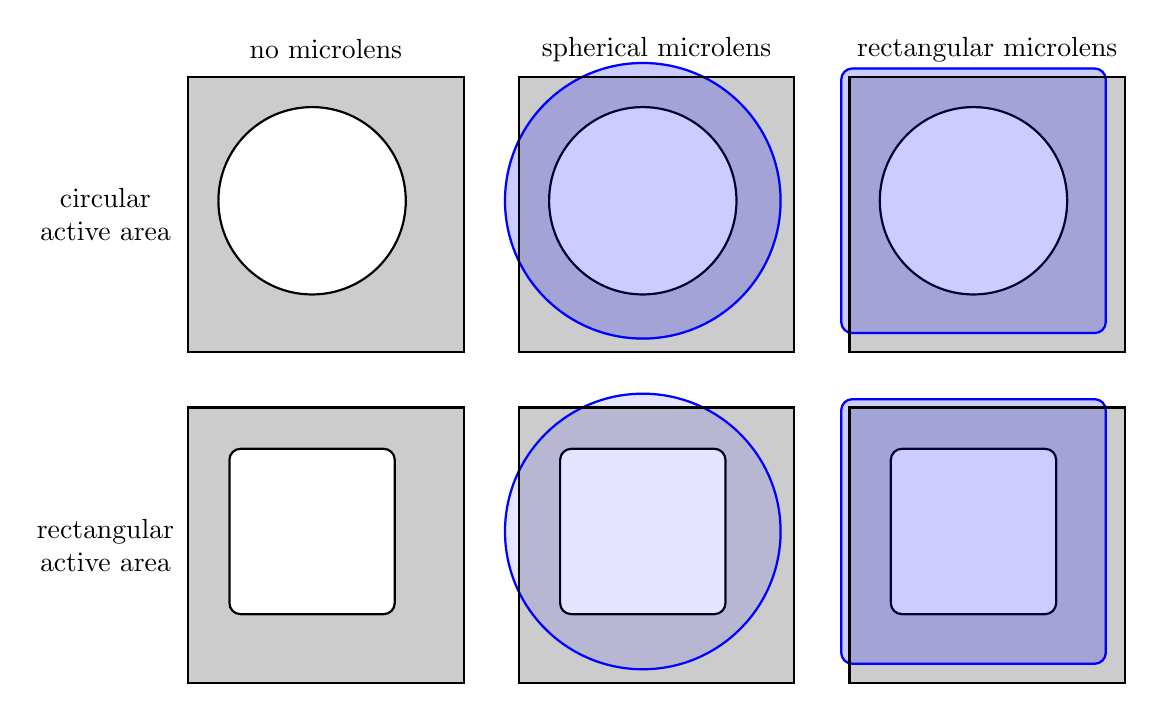
\begin{tikzpicture}[thick,scale=0.7, every node/.style={scale=1}]

\draw[fill, color=black!20]  (-1.25,3.25) rectangle (3.75,-1.75);
\draw[fill, color=white]  (1,1) ellipse (1.7 and 1.7);
\draw[]  (1,1) ellipse (1.7 and 1.7);

\draw[fill, color=black!20]  (4.75,3.25) rectangle (9.75,-1.75);
\draw[fill, color=white]  (7,1) ellipse (1.7 and 1.7);
\draw[]  (7,1) ellipse (1.7 and 1.7);
\draw [fill, color=blue, opacity=0.2] (7,1) ellipse (2.5 and 2.5);
\draw [color=blue] (7,1) ellipse (2.5 and 2.5);

\draw[fill, color=black!20]  (10.75,3.25) rectangle (15.75,-1.75);
\draw[fill, color=white]  (13,1) ellipse (1.7 and 1.7);
\draw[]  (13,1) ellipse (1.7 and 1.7);
\draw [fill, color=blue, opacity=0.2, rounded corners] (10.6,3.4) rectangle (15.4,-1.4);
\draw [color=blue, rounded corners] (10.6,3.4) rectangle (15.4,-1.4);

\draw[fill, color=black!20]  (-1.25,-2.75) rectangle (3.75,-7.75);
\draw[fill, color=white, rounded corners] (-0.5,-3.5) rectangle (2.5,-6.5) {};
\draw[rounded corners] (-0.5,-3.5) rectangle (2.5,-6.5) {};

\draw[fill, color=black!20]  (4.75,-2.75) rectangle (9.75,-7.75);
\draw[fill, color=white, rounded corners] (5.5,-3.5) rectangle (8.5,-6.5) {};
\draw[rounded corners] (5.5,-3.5) rectangle (8.5,-6.5) {};
\draw [fill, color=blue, opacity=0.1] (7,-5) ellipse (2.5 and 2.5);
\draw [color=blue] (7,-5) ellipse (2.5 and 2.5);

\draw[fill, color=black!20]  (10.75,-2.75) rectangle (15.75,-7.75);
\draw[fill, color=white, rounded corners] (11.5,-3.5) rectangle (14.5,-6.5) {};
\draw[rounded corners] (11.5,-3.5) rectangle (14.5,-6.5) {};
\draw [fill, color=blue, opacity=0.2, rounded corners] (10.6,-2.6) rectangle (15.4,-7.4);
\draw [color=blue, rounded corners] (10.6,-2.6) rectangle (15.4,-7.4);

\draw[]  (-1.25,3.25) rectangle (3.75,-1.75);
\draw[]  (4.75,3.25) rectangle (9.75,-1.75);
\draw[]  (10.75,3.25) rectangle (15.75,-1.75);

\draw[]  (-1.25,-2.75) rectangle (3.75,-7.75);
\draw[]  (4.75,-2.75) rectangle (9.75,-7.75);
\draw[]  (10.75,-2.75) rectangle (15.75,-7.75);

\node at (1.25,3.75) {no microlens};
\node at (7.25,3.75) {spherical microlens};
\node at (13.25,3.75) {rectangular microlens};
\node[align=center] at (-2.75,0.75) {circular\\active area};
\node[align=center] at (-2.75,-5.25) {rectangular\\active area};
\end{tikzpicture}
    \caption{Options for lenses with varying types of active areas and microlenses}
    \label{tkz:SPAD_types}
\end{figure}


The use of microlenses is not the only viable of option of increasing the active area on the chip. A second option is to pick the circuitry required per SPAD, and push it to the side. These circuitry include the Read-Out Integrated Circuit (ROIC) that also includes the quenching of the SPADs, and the Time interval to Digital converter (TDC). 

To avoid pileup, the following calculations are done for an $0.18\,\mu m$ technology and it is assumed that the ROIC will take up $110\,\mu m^2$ surface area per SPAD, and that the TDC will take up $1200\,\mu m^2$ surface area per SPAD. It will also be assumed that the minimum amount of pitch between two SPADs is $1.5\,\mu m$. These numbers are based on current SPAD designs in $0.18\,\mu m$ technology. An overview of the performance of all different possibilities is shown in \cref{fig:effective_area}.

% \begin{figure}[h]
% \centering
% 	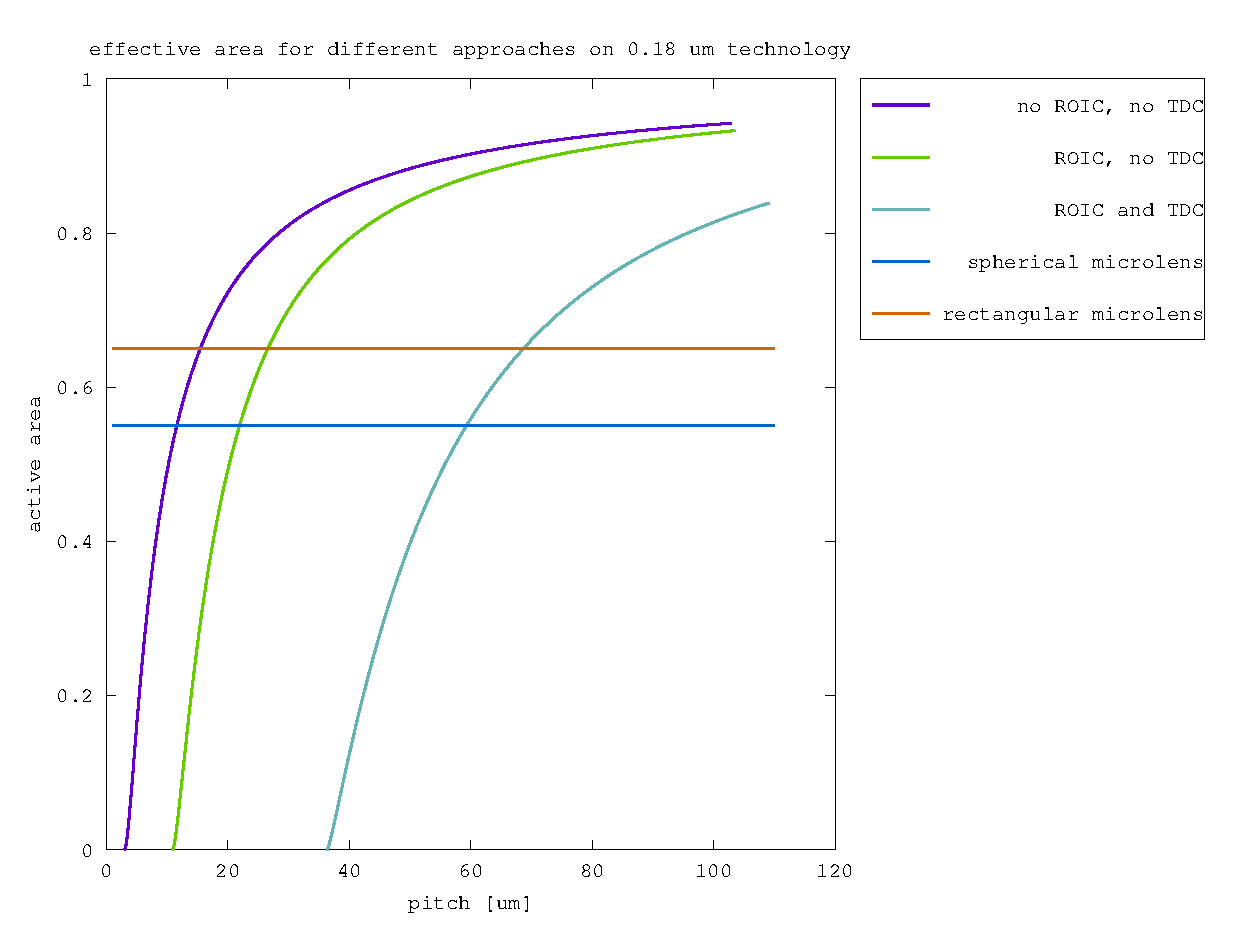
\includegraphics[width=0.8\linewidth]{fig/effective_area.eps}
% \caption{effective area for different approaches in relationship to the pitch of the SPAD on $0.18\,\mu m$ technology}
% \label{fig:effective_area}
% \end{figure} 


\section{Detected photon characterisation}\label{ssec:HDM_detected_photon_characterisation}
This section is similar to \cref{ssec:detected_photon_characterisation}, but recalculates parts that are different for the HDM mode. First of all, the results of all the SPAD measurements are no longer bundled together, but interpreted seperately. Also the device is a lot closer to Europa with an altitude of at most $500\,m$ which causes the laser to be me more effective when compared to the noise. The new values to work with are shown in \cref{tab:photons_per_SPAD}. Note that the $PPS_S$ is the amount of photons per Watt of optical transmitted energy.


\begin{table}[H]
\centering
\caption{Amount of backgroun (B), dark count (N), and signal (S) photons that hit a single SPAD per second}
\label{tab:photons_per_SPAD}
\begin{tabular}{|l|r|}\hline
    \textbf{photons per SPAD} & \\
    \hline 
    $PPS_B$ & $3.54\cdot10^{8}\,\text{photon}/s$ \\
    $PPS_N$ & $2.00\,k \text{photon}/s$ \\
    $PPS_S$ & $9.39\,k \text{photon}/s$ \\
    \hline 
\end{tabular}
\end{table}


Another important changed property, is that the maximum time of flight $t_{round}=3.33\,\mu s$. This directly means that per measurement, less noise is received. However, the expected amount of noise per bin remains the same. The new $\mu_n=\frac{3.33\cdot10^{-6}}{2}=1.67\,\mu s$, and the new $\sigma_n=\frac{3.33\cdot10^{-6}}{\sqrt{12}}=304\,ns$. 

\section{Required laser power}\label{ssec:HDM_required_laser_power} The laser power too requires new calculations when compared to those performed in \cref{ssec:required_laser_power}. First and foremost, the resolution required for the Hazard Detection Mode is $5\,cm$, with a resulting maximum allowable standard deviation of $\sigma_{tot}=142\,ps$. Finally, it was decided that a scanning method would be used where the target area would be divided into at least $2048/8=256$ pieces. \Cref{fig:hdm_s_vs_n} and \cref{fig:hdm_s_vs_n_small} show the updated relationship between signal and noise photons to meet the requirements.

\begin{figure}[h]
\centering
	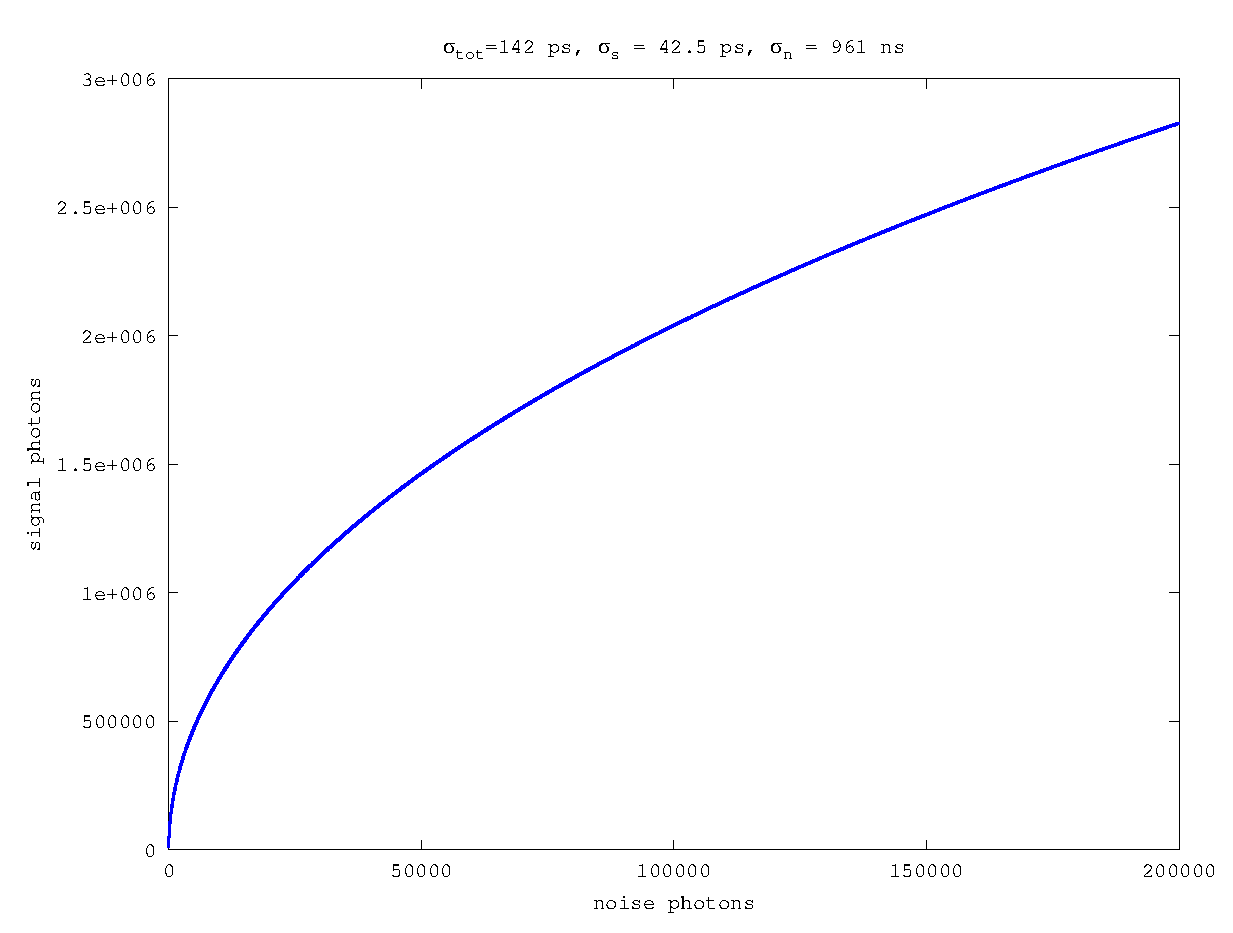
\includegraphics[width=0.8\linewidth]{fig/hdm_s_vs_n.eps}
\caption{required signal photons for a given number of noise photons to meet the HDM requirements at maximum altitude}
\label{fig:hdm_s_vs_n}
\end{figure}

\begin{figure}[h]
\centering
	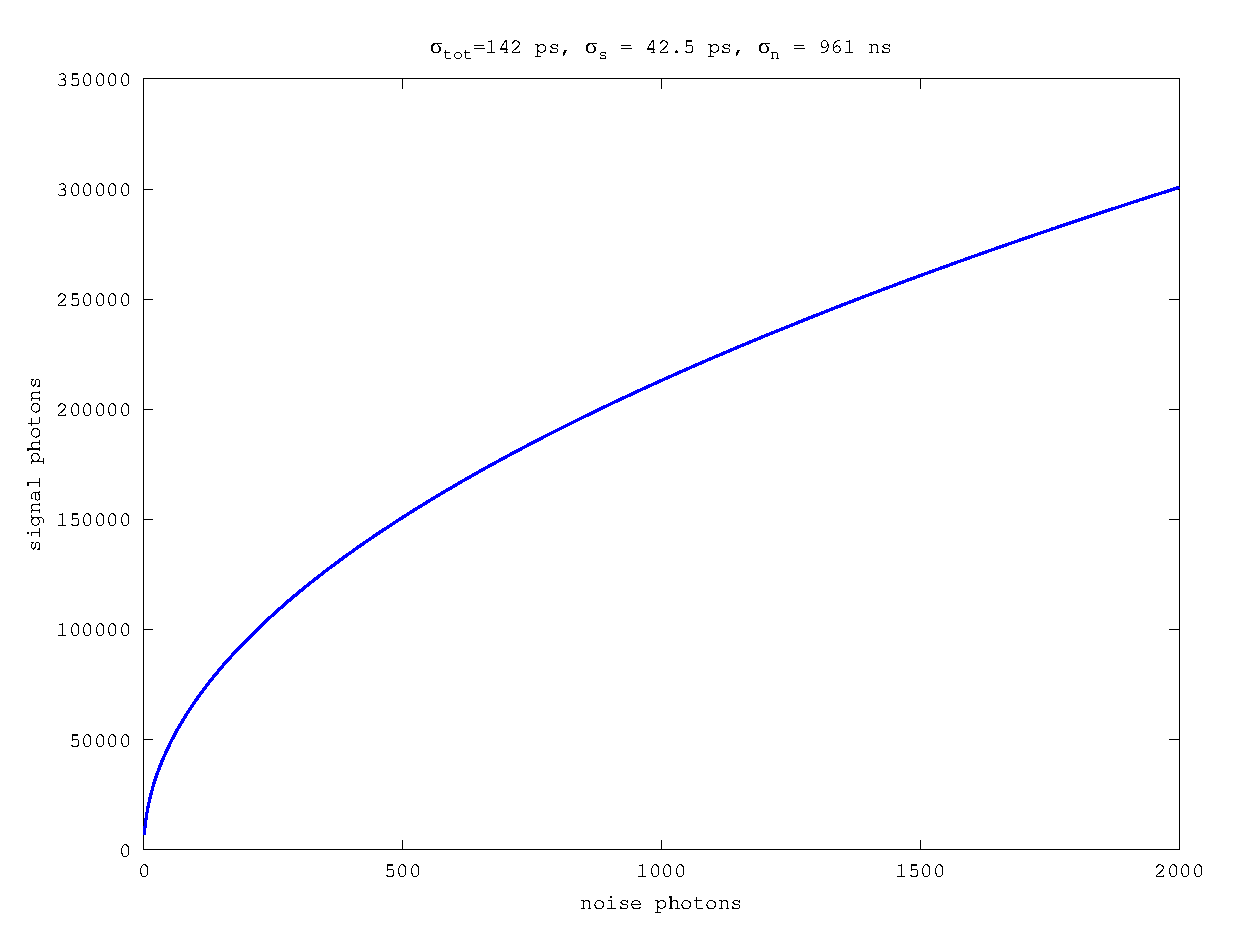
\includegraphics[width=0.8\linewidth]{fig/hdm_s_vs_n_small.eps}
\caption{required signal photons for a given number of noise photons to meet the HDM requirements at maximum altitude}
\label{fig:hdm_s_vs_n_small}
\end{figure}

All the acquired new information can now be used to calculate a new relationship between the required peak power and average power. Note that in this case the least amount of pulses is 256. The reason being oly a 1/256th of the target can be observed at a time. The results of these calculations are shown in \cref{fig:hdm_peak_vs_av}. This time increasing the number of pulses does decrease the required signal power significantly. The more important result is however, that the power budget is orders of magnitude of for obtaining a feasible peak optical power for the laser. Therefore the HDM modus is not feasible without extra processing like an energy threshold.

\begin{figure}[h]
\centering
	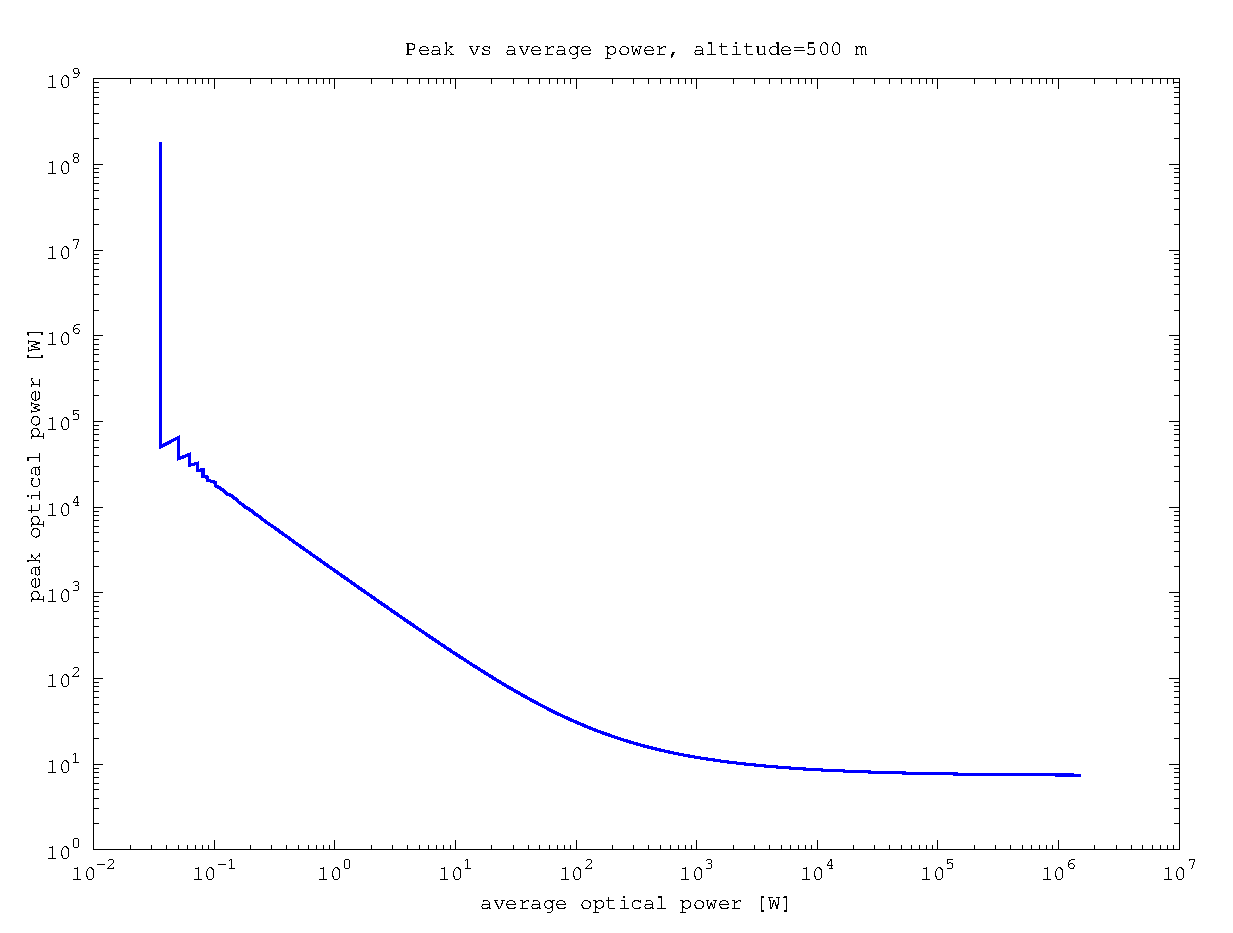
\includegraphics[width=0.8\linewidth]{fig/hdm_peak_vs_av.eps}
\caption{required signal photons for a given number of noise photons to meet the HDM requirements at maximum altitude}
\label{fig:hdm_peak_vs_av}
\end{figure}

The next step is to look at the energy threshold again. The average noise power $P_B=7.4\,W$. In order to make sure that the expected amount of photons per bin is 10 times higher than for the noise, one needs a peak power of $P_{peak}=74\,W$. The resulting average optical laser power is calculated below.

\begin{align*}
	P_{av}&=P_{peak}\cdot\frac{2048}{8}\cdot FWHM\\
	&= 74\cdot256\cdot100\cdot10^{-12}\\
	&= 1.89\,\mu W
\end{align*}

Both the peak and average laser power fall royally in the power budget. This means that the device can meet the resolution requirements within the power budget, granted that the damage caused by radiation can be reasonably contained. This will be investigated in \cref{sec:radiation}. Another important, but less pressing challenge is the design of the readout and the data processing of the SPAD array. 


\clearpage
\section{Readout}\label{ssec:readout}
In \cref{ssec:SPADs} two circuitry components where mentioned that are required for each SPAD: a ROIC and a TDC. While the decision on whether or not to push out the ROIC has not yet been made, \cref{ssec:SPAD_layout} concluded that it is necessary to push out the TDC. One other important aspect of the TDC is that it must meet the designed resolution of $50\,ps$. The proposed TDC design uses a Phase Locked Loop (PLL) to generate signals that the TDC can use to timestamp an incomming pulse. The PLL, for which a schematic is shown in \cref{tkz:PLL}, locks onto an input in such a way, that both signals entering te phase detector are equal. By using a divider by $X$ block, one can generate a signal with a frequency that is equal to $x$ times the clock frequency. The voltage controlled oscilator is capable of generating 4 signals with 4 different phases to increase the resolution further. \Cref{tkz:TDC_line_PLL} shows a line of TDCs connected to the PLL.
		
\begin{figure}[H]
    \centering

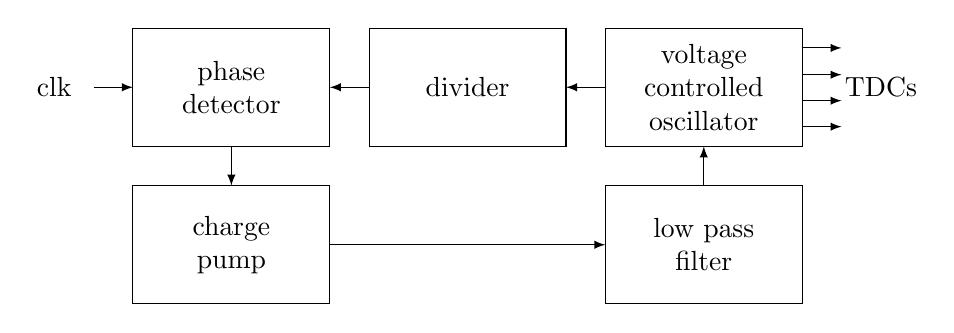
\begin{tikzpicture}

\draw  (-2,1.75) rectangle (0.5,0.25) node[pos=.5, align=center]{phase\\detector};
\draw  (1,1.75) rectangle (3.5,0.25) node[pos=.5, align=center]{divider};
\draw  (4,1.75) rectangle (6.5,0.25) node[pos=.5, align=center]{voltage\\controlled\\oscillator};
\draw  (4,-0.25) rectangle (6.5,-1.75) node[pos=.5, align=center]{low pass\\filter};
\draw  (-2,-0.25) rectangle (0.5,-1.75) node[pos=.5, align=center]{charge \\pump};

\draw [>=latex, ->] (1,1) -- (0.5,1);
\draw [>=latex, ->] (4,1) -- (3.5,1);
\draw [>=latex, ->] (0.5,-1) -- (4,-1);
\draw [>=latex, ->] (-0.75,0.25) -- (-0.75,-0.25);
\draw [>=latex, ->] (5.25,-0.25) -- (5.25,0.25);
\draw [>=latex, ->] (-2.5,1) -- (-2,1);

\draw [>=latex, ->] (6.5,1.5) -- (7,1.5);
\draw [>=latex, ->] (6.5,1.16) -- (7,1.16);
\draw [>=latex, ->] (6.5,.83) -- (7,.83);
\draw [>=latex, ->] (6.5,0.5) -- (7,0.5);


\node at (-3,1) {clk};
\node at (7.5,1) {TDCs};
\end{tikzpicture}
    \caption{schematic of phase locked loop generating signals for TDCs}
    \label{tkz:PPL}
\end{figure}

\begin{figure}[H]
    \centering


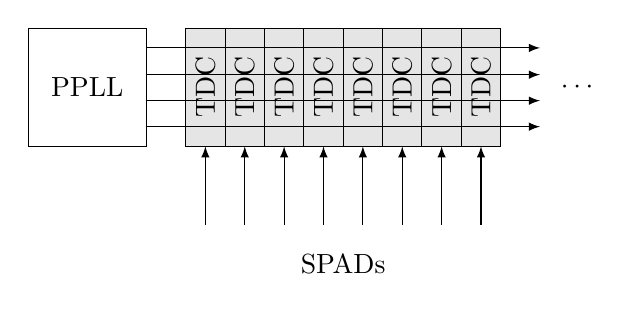
\begin{tikzpicture}

\draw  (-3.25,3) rectangle (-1.75,1.5) node[pos=.5]{PPLL};

\draw [fill=gray!20] (-1.25,3) rectangle (-0.75,1.5) node[pos=.5, rotate=90]{TDC};
\draw [fill=gray!20] (-0.75,3) rectangle (-0.25,1.5) node[pos=.5, rotate=90]{TDC};
\draw [fill=gray!20] (-0.25,3) rectangle (0.25,1.5) node[pos=.5, rotate=90]{TDC};
\draw [fill=gray!20] (0.25,3) rectangle (0.75,1.5) node[pos=.5, rotate=90]{TDC};
\draw [fill=gray!20] (0.75,3) rectangle (1.25,1.5) node[pos=.5, rotate=90]{TDC};
\draw [fill=gray!20] (1.25,3) rectangle (1.75,1.5) node[pos=.5, rotate=90]{TDC};
\draw [fill=gray!20] (1.75,3) rectangle (2.25,1.5) node[pos=.5, rotate=90]{TDC};
\draw [fill=gray!20] (2.25,3) rectangle (2.75,1.5) node[pos=.5, rotate=90]{TDC};

\draw [>=latex, ->] (-1.75,2.75) -- (3.25,2.75);
\draw [>=latex, ->] (-1.75,2.41) -- (3.25,2.41);
\draw [>=latex, ->] (-1.75,2.08) -- (3.25,2.08);
\draw [>=latex, ->] (-1.75,1.75) -- (3.25,1.75);

\draw [>=latex, ->] (-1,0.5) -- (-1,1.5);
\draw [>=latex, ->] (-0.5,0.5) -- (-0.5,1.5);
\draw [>=latex, ->] (0,0.5) -- (0,1.5);
\draw [>=latex, ->] (0.5,0.5) -- (0.5,1.5);
\draw [>=latex, ->] (1,0.5) -- (1,1.5);
\draw [>=latex, ->] (1.5,0.5) -- (1.5,1.5);
\draw [>=latex, ->] (2,0.5) -- (2,1.5);
\draw [>=latex, ->] (2.5,0.5) -- (2.5,1.5);

\node at (3.75,2.25) {$\cdots$};
\node at (0.75,0) {SPADs};
\end{tikzpicture}
    \caption{TDC line connected to PLL}
    \label{tkz:TDC_line_PLL}
\end{figure}

\subsection{Histogram}
Depending on whether an energy threshold is used or not, the data must be stored in a histogram. If no energy threshold is needed, one can simply add all the timestamps together and devide by the amount of oberserved counts to get a simple  average. For more sophisticated signal processing however, more data needs to be transferred to the FPGA than just an average. One can either read every TDC value directly into the FPGA, but for the expected amount of traffic, this  is not feasable. Therefore a histogram is necessary to condense the data into a smaller package without losing essential information. Considering that a histogram will be needed for every SPAD, the amount of space on the chip that the histograms can turn out to be quite large. 

The amount of bits required per SPAD are dependent on the binzise, resolution and bandwidth, and can be calculated using \cref{eq:histogram_bits}. 

\begin{equation}
		\text{bits} = \text{SPADs}\cdot\lceil \log_2(\text{binsize}) \rceil\cdot \lceil \frac{\text{bandwidth}}{\text{resolution}}\rceil
		\label{eq:histogram_bits}
\end{equation}

The next step is to investigate the limitations of these variables. First of all, the resolution is very important for both the accuracy of the device and the performance of the energy detection. The latter has a direct relationship with the power of the laser. Lowering the resolution will effectively decrease the peak power of the signal, because the power is effectively distributed over the length of a single bin. It is assumed that the FWHM of the laser is $100\,ps$i. So in order to ensure that at least one bin is exposed to the signal pulse in it's entire duration, one needs a resolution of $50\,ps$. This is also the resolution that is considered for the TDC. The binsize is dependedent on the light intensity, which will increase when approaching Europa. The bandwidth allows for some flexibility. For example, when the previous measurements where close to 8 km the device can't travel far from that altitude in the next second. The next measurement will most likely also not yield an altitude further away than the previous one. Therefore the bandwidth can be limited to some extend, and adjusted between measurements.

\subsection{On chip signal processing}
When a histogram is constructed one can decide to process the data on the chip before sending it to the FPGA. This limits the complexity of the processingstep however. It is difficult to implement a reasonable dynamic threshold for every individual histrogram, and more complex waveforms that utilize known characteristics of the signal and noise photons other than intensity becomes infeasable. However a simple circuit that only sends the largest peak, or eliminates all values before the threshold is possible. 

\subsection{connection to FPGA}
The information stored in the histograms needs to be transported to the FPGA. There are several approaches that can be used to do this. 



\chapter{Radiation}\label{sec:radiation}
One of the key challenges for deploying a sensor on the Europa Clipper is it's resilience on large amounts of radiation. The performance of the SPAD technology considered in this report when exposed to large amounts of radiation must therefore be examined.

\section{linoSPAD}\label{ssec:linoSPAD}
F
To characterise the performance of the $0.18\,\mu s$ technology SPADs. The LinoSPAD as developed by Sammuel Burri et al. features a SPAD array of this type \cite{burri2016linospad}. therefore the LinoSPAD was used to test it's resilience against radiation. \Cref{tkz:schematic_linoSPAD} shows a simple schematic of the linoSPAD. Note that the SPAD array is isolated from the readout electronics and FPGA. This is convenient for testing with a radiation beam that can be that can be directed to the SPAD array and away from the sensitive ROIC and FPGA. This layout is also useful to shield of the ROIC and FPGA using e.g. blocks of lead.

\begin{figure}[H]
    \centering


\begin{tikzpicture}

\draw  (-2,3) rectangle (2.5,-5) node[pos=.5]{};
\draw  (-1.5,-1) rectangle (2,-4.5) node[pos=.5, align=center]{\large ROIC\\\large$+$\\\large FPGA};
\draw  (0,2) rectangle (0.5,0) node[pos=.5, rotate=90]{SPAD array};

\draw [>=latex, ->] (3,-3.5) -- (2.5,-3.5);
\draw [>=latex, ->] (2.5,-1) -- (3,-1);
\draw [>=latex, ->] (-2.5,0) -- (-2,0);

\node[align=center] at (-3,0) {power\\FPGA};
\node[align=center] at (3.5,-1) {data\\out};
\node[align=center] at (3.5,-3.5) {power\\SPADs};
\end{tikzpicture}
    \caption{simple schematic of linoSPAD}
    \label{tkz:schematic_linoSPAD}
\end{figure}

The software used to read out the linoSPAD is programmed to count the photons for each individual SPAD for a duration of one second and store this information in a file. This operation is called every minute.

\section{Test setup}\label{ssec:test_setup}
To characterise the performance of the linoSPAD under radiation, a test was performed in the cylcotron of the Paul Screrrer Institute (PSI) in Switzerland. The test involved proton radiation beams of both $60\,MeV$ and $10.1\,MeV$. A schematic of the setup is shown in \cref{tkz:test_setup}. The collimator and radiation shield have to make sure that only the SPAD array gets a large radiation dose. \Cref{fig:dosis} shows the amount of radiation that is projected onto the SPAD array as a function of time. The red dashed lines indicate the start and stop time of the $60\,MeV$ beam, and the green dashed lines indicate the start and stop of the $10\,MeV$ beam. The collimator eeds to be replaced when switching from $60\,MeV$ to $10\,MeV$ which is why the power of the SPAD array will be off for a brief time during the test. The blue line indicates the moment the power of the SPAD array is off.

\begin{figure}[H]
    \centering



\begin{tikzpicture}

\draw  (-6,-5.5) rectangle (5,-6) node[pos=.5]{circuitboard};
\draw  (0,-5) rectangle (4.5,-5.5)node[pos=.5]{ROIC and FPGA};
\draw  (-4.5,-5) rectangle (-2.5,-5.5)node[pos=.5]{SPADs};

\draw (5.5,-4) -- (-1,-4) -- (-1,-2.5) -- (5.5,-2.5);

\node at (2.5,-3.25) {radiation shield};

\draw [>=latex, ->] (-3.5,2) -- (-3.5,-5);
\node at (-3.5,2.5) {proton beam};
\draw  (-8.5,0) rectangle (-3.75,-1) node[pos=.5]{collimator};
\draw  (-3.25,0) rectangle (1.5,-1) node[pos=.5]{collimator};

\draw [>=latex, ->] (-3.6,2) -- (-3,0);
\draw [>=latex, ->] (-3.7,2) -- (-3.8,0);
\draw [>=latex, ->] (-3.4,2) -- (-3.75,-.5);
\draw [>=latex, ->] (-3.45,2) -- (-3.65,-5);

\end{tikzpicture}


    \caption{schematic of radiation test setup}
    \label{tkz:test_setup}
\end{figure}




\begin{figure}[h]
\centering
	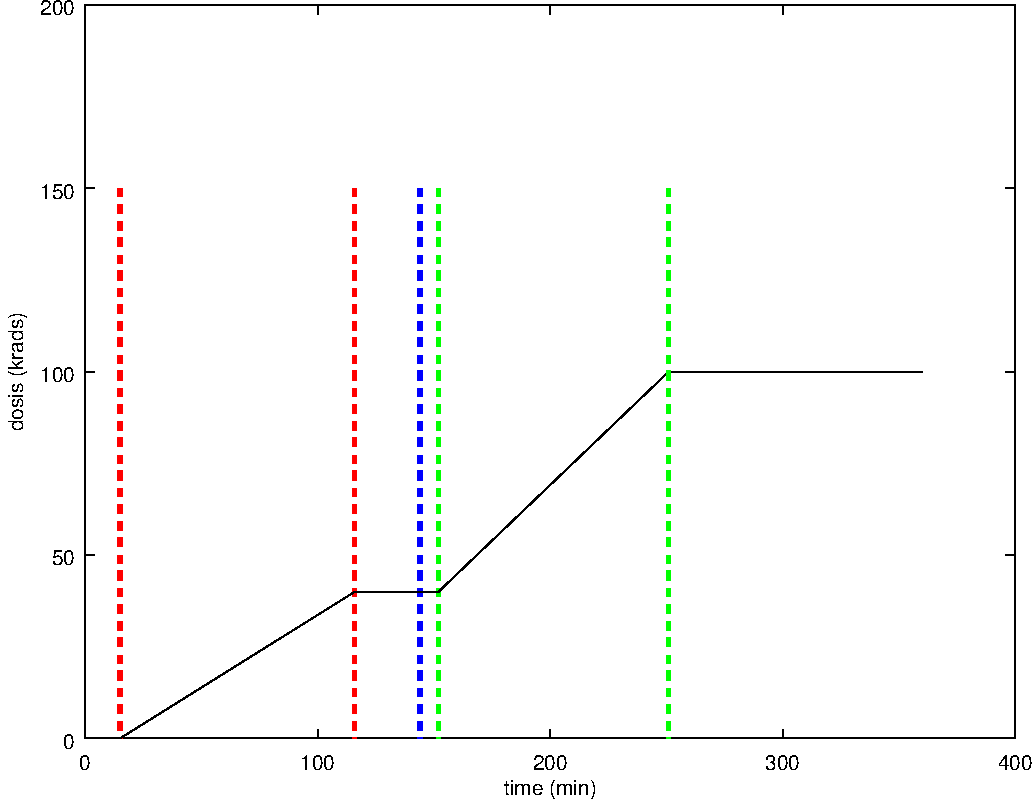
\includegraphics[width=0.6\linewidth]{fig/dosis.pdf}
\caption{The accumulative dose of radiation produces by the proton radiance as a function of time}
\label{fig:dosis}
\end{figure}



\clearpage
\section{Measurements}\label{ssec:results}
This section shows the measurents and results obtained during the radiation experiment. Note that the linoSPAD used is a relatively noise one, in the knowledge that the device  would no longer be usable for normal applications after the radtiation test.

\Cref{fig:count_vs_time_sum_all} shows the accumulative DCR of all SPADs as a function of time. The first 150 minutes are behaving as expected. The plot shows that the DCR linearly increases when the $60\,MeV$ beam  is turned on with a constant intensity. After the beam is turned off, the DCR stops rising and the device starts annealing, resulting in a gradual derease of the DCR. A approximately 145 minutes, the device receives a total of 0 counts, and the reason for that is that the power on the SPAD array was briefly tunred off at that time. However the device behaves unexpectedly when the $10\,MeV$ beam is turned on. There is no change in DCR that can be observed due to the $10\,MeV$ beam, which is cotnradictory with the expectations that the $10\,MeV$ beam would cause more damage than the $60\,MeV$ beam. Another interesting event is that at approximately 165 minutes, $25\,\%$ of the SPADs no longer detect counts. \Cref{fig:count_vs_time_sum_some} shows the same graph, but with the $25\,\%$ defect SPADs removed. Here one can see that the other SPADs are not at all affected by the $10\,MeV$ beam and continue annealing. At approximately 240 minutes the entire sensor stops communicating, 10 minutes before the beam is turned off.



\begin{figure}[h]
\centering
	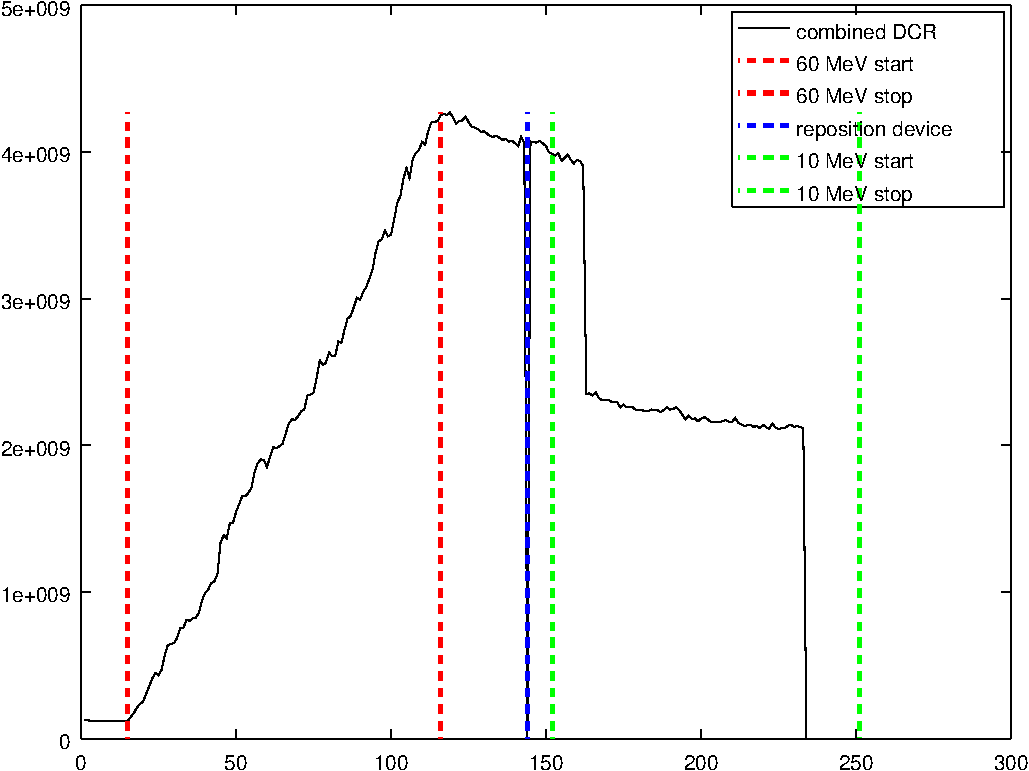
\includegraphics[width=0.6\linewidth]{fig/count_vs_time_sum_all.pdf}
\caption{The amount of DCR for the sum of all SPADs combined as a function of time}
\label{fig:count_vs_time_sum_all}
\end{figure}


\begin{figure}[h]
\centering
	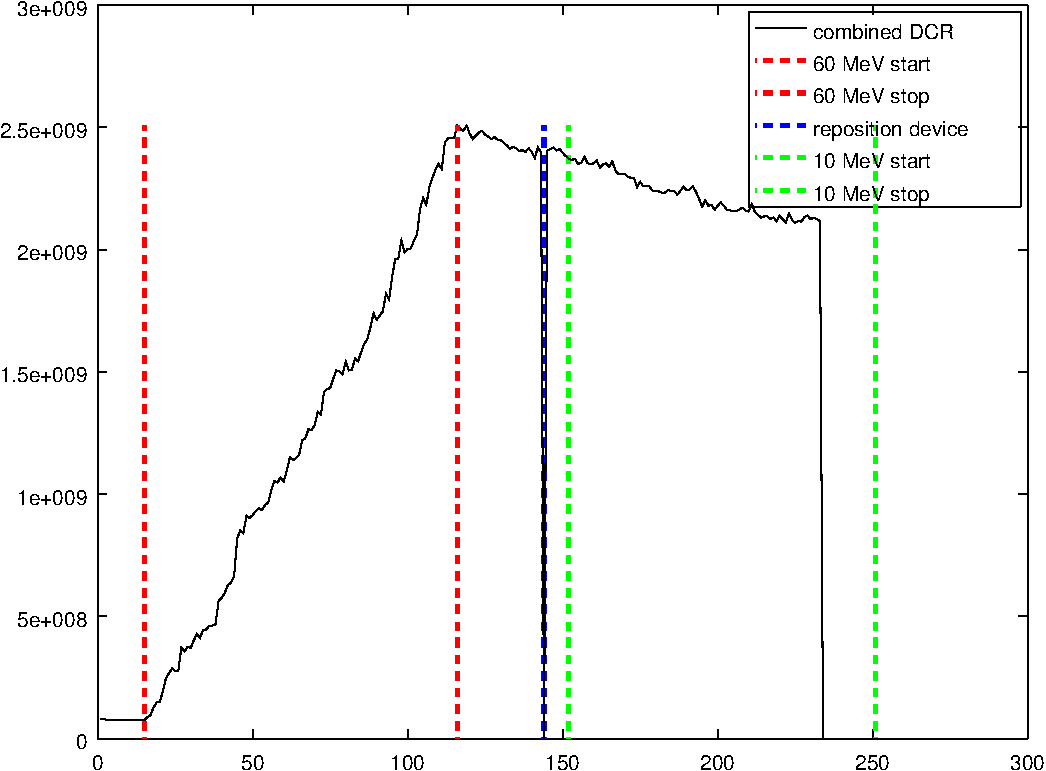
\includegraphics[width=0.6\linewidth]{fig/count_vs_time_sum_some.pdf}
\caption{The amount of DCR for the sum of $75\,\%$ of SPADs combined as a function of time. The left-out $25\,\%$ are the SPADs that broke down at the 165 minute mark}
\label{fig:count_vs_time_sum_some}
\end{figure}

\Cref{fig:bars} shows the accumulative number of counts for individual SPADs. This plot illustrates that the contribution in DCR varies wildly across different SPADs. It also shows that the second half of the SPADs seem te behave at a much lower count than the first half, which is something that needs to be looked at.

\begin{figure}[h]
\centering
	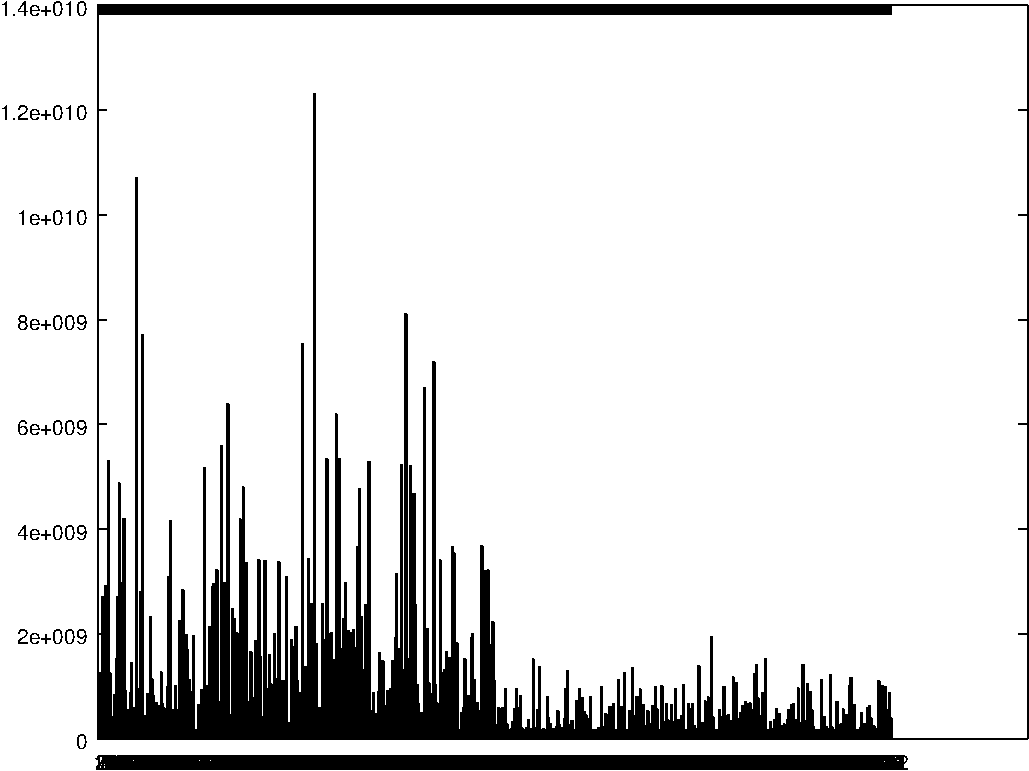
\includegraphics[width=0.6\linewidth]{fig/bars.pdf}
\caption{accumulative number of counts for the entire experiment for individual SPADs}
\label{fig:bars}
\end{figure}

\Cref{fig:spad_high}, \cref{fig:spad_mid} and \cref{fig:spad_low} show the individual DCR as a function of time for three SPADs in the high, mid and low segment respectively. The segments are sorted by how much counts a SPAD accumulated over the course of the entire test. Note that the individual SPADs don't show the same trend as the sum of all SPADs. The individual SPADs get damaged at arbitray points in time, and anneal at a certain point in time. 

\begin{figure}[h]
\centering
	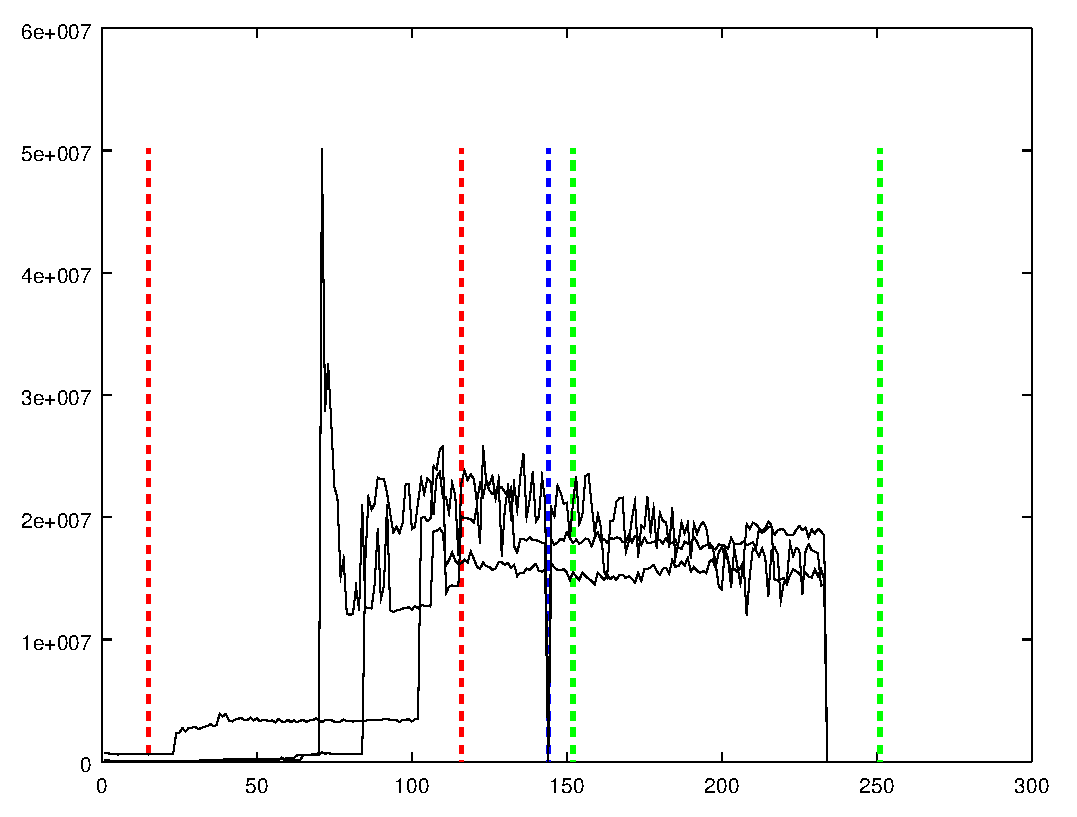
\includegraphics[width=0.6\linewidth]{fig/spad_high.eps}
\caption{three SPADs from that are in picked from the $33\,\%$ SPADs with the highest contribution to noise}
\label{fig:spad_high}
\end{figure}


\begin{figure}[h]
\centering
	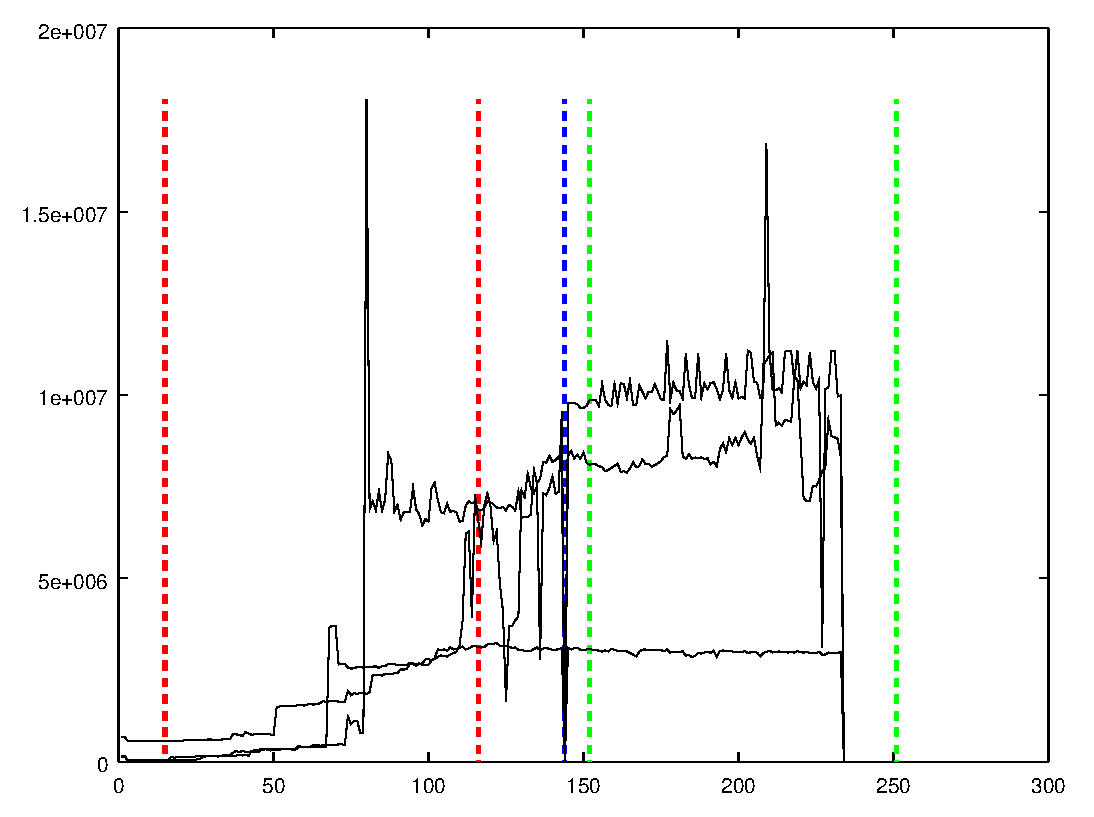
\includegraphics[width=0.6\linewidth]{fig/spad_mid.eps}
\caption{three SPADs from that are in picked from the $33\,\%$ SPADs with the most average contribution to noise}
\label{fig:spad_mid}
\end{figure}


\begin{figure}[h]
\centering
	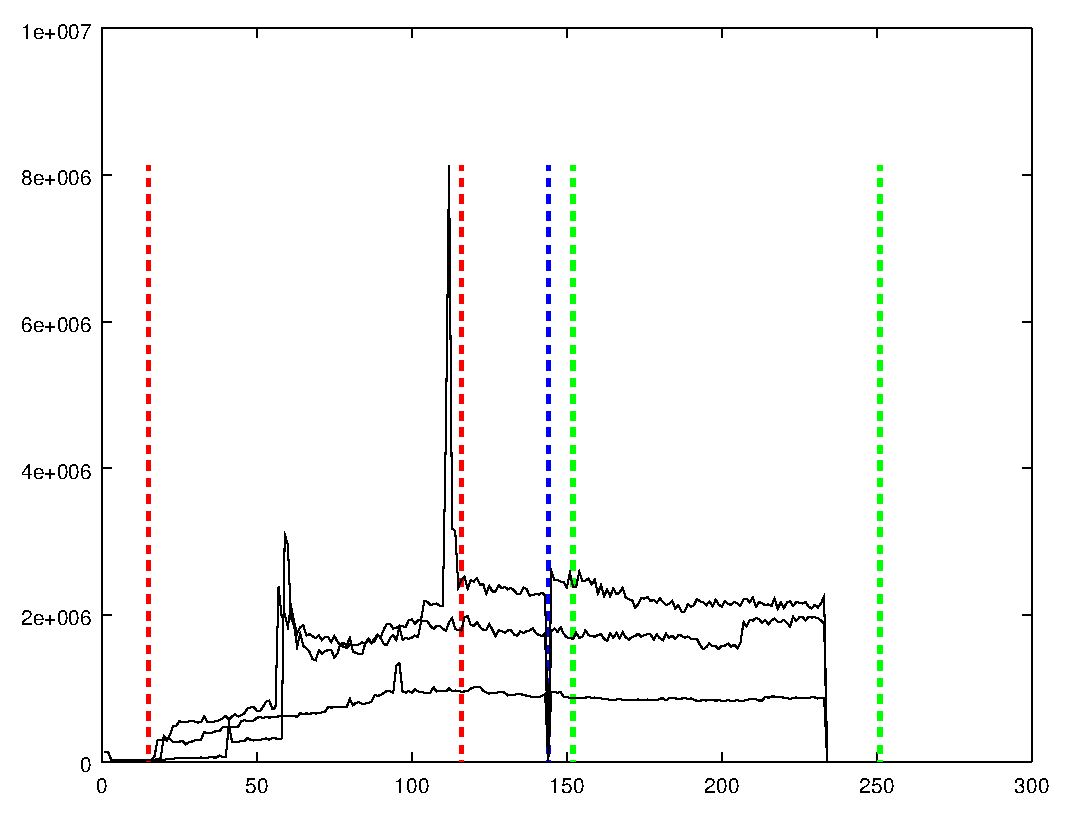
\includegraphics[width=0.6\linewidth]{fig/spad_low.eps}
\caption{three SPADs from that are in picked from the $33\,\%$ SPADs with the lowest  contribution to noise}
\label{fig:spad_low}
\end{figure}

\Cref{fig:sigmoid_sweep} shows the spread of DCR for single SPADs at different points in time. The behavior is consistent with the results shown in \cref{fig:count_vs_time_sum_all}. Note that after approximately 165 minutes $25\,\%$ of the SPADs stop working, which is the reason why the black line starts at $25\,\%$.

\begin{figure}[h]
\centering
	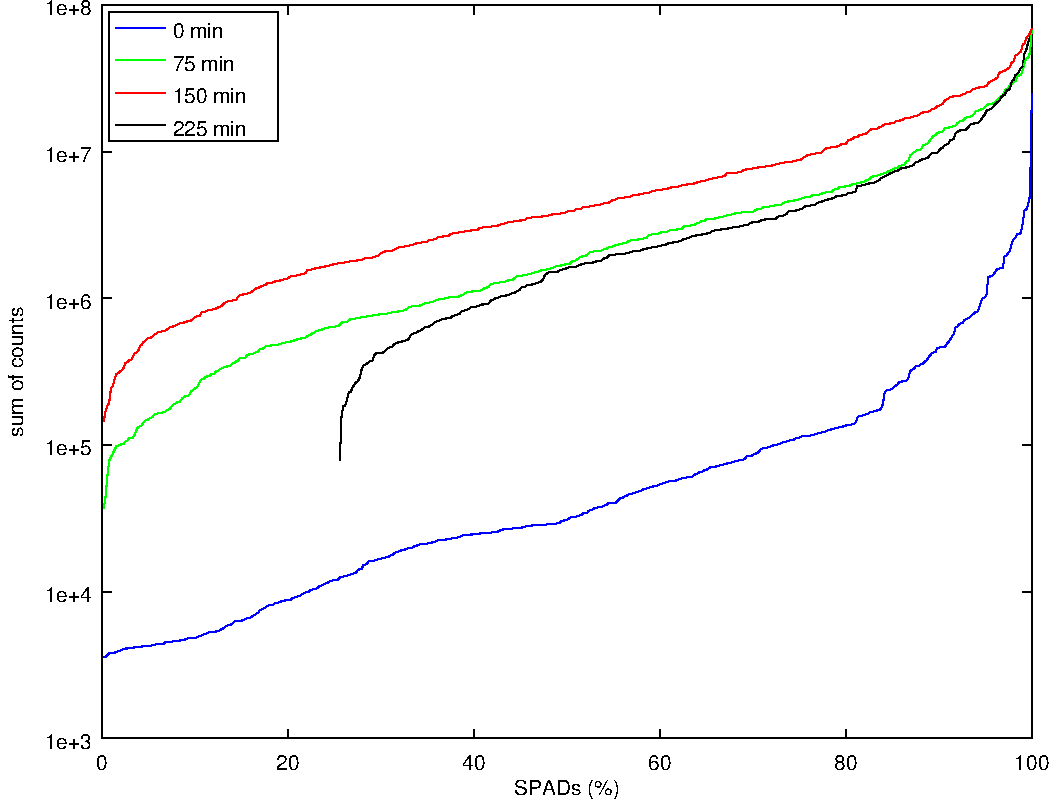
\includegraphics[width=0.6\linewidth]{fig/sigmoid_sweep.pdf}
\caption{distribution of DCR over individual SPADs at different time frames. After the 165 minute mark $25\,\%$ of SPADs stop working, which is why the black line starts later at $25\,\%$}
\label{fig:sigmoid_sweep}
\end{figure}


The results of the test are in line with until the 150 minute mark, but afterwards the reaction to the $10\,MeV$ beam is odd. The break down at 165 minutes and 250 minutes indicate damage in the readout circuit. This is a feasible explanation for the events as it is known that the $10\,MeV$ can be very damaging to these types of cicruitry. This would mean that the protection provided for the ROIC and FPGA where insufficient. There are two possible explanations for the observation that the SPADs are not affected by the $10\,MeV$ beam that will be listed here. The first explanation, is that the SPADs at this particular $0.18\,\mu m$ technology are not affected by the $10\,MeV$ as opposed to their $0.35\,\mu m$ counterpart. The second explanation is that something went wrong during the setup of the $10\,MeV$ beam test, which caused the beam to aim for the ROIC and FPGA instead of the SPAD array. 

Considering only the effect of the $60\,MeV$ beam, and especially the behavior observed in \cref{fig:count_vs_time_sum_some}, show a very interesting trend where the change in DCR seems to be a linear relationship with the amount of radiation it is exposed to. Both the periods between 10 and 120 minutes, and between 120 and 240 minutes show a very constant slope. This means that not only the amount, but also the time over which the radiation dose is accumulated graetly affects the DCR of the device. This property should be further investigated and compared to the circumstances at Europa.

\clearpage
\section{Comparison}\label{ssec:results}

The next step is to compare the results from the measurements obtained in this experiment, and results from precious experiments. An overview of the performance of this device when compared to another with $3.5\,\mu m$ technology is shown in \cref{tab:comparison}. The measurements of the compared device are based on the work of Carrara et al. \cite{carrara2009gamma} and Burri \cite{burri2016thesis}. A first observation is that the DCR of the new measurements show DCR measurements that are way higher than the other devices. There are three possible explanations for this. Firstly, in the knowledge that the device would be unusable after the test, a relatively noise device was used. Secondly, the SPADs used in the new device have a lot more active area that is capable of receiving photons, but also receive radiation, generate DCR and traps. A third possibility is an error in the software where the DCR does not match the read-out values. Consistent. Also the effect of radiation is different. The old measurements show an increase of roughly 50 times the DCR, while the new test shows an increase of 250 times.

\begin{table}[h]
		\centering
\caption{Comparison of DCR for different radiation tests. The bold entry is the one described in this report}
\label{tab:comparison}
\begin{tabular}{|ll|lll|} \hline
\textbf{proton energy} & dose             & initial DCR       & final DCR         & DCR after annealing (anneal time) \\ \hline
10 Mev                 & 40 krad          & 140               & 6298              & 3884 (10 days)                    \\
60 Mev                 & 40 krad          & 142               & 6290              & 1299 (21 days)                    \\
\textbf{60 Mev}        & \textbf{40 krad} & $\mathbf{2\cdot10^4}$ & $\mathbf{5\cdot10^6}$ & $\mathbf{4\cdot10^6 \textbf{(2 hours)}}$      \\  \hline
\end{tabular}
\end{table}

There are two considerations to be made on these observations. The first one is to redo the measurements to confirm them. The measurements don't line up with the expectations, especially for the $10\,MeV$ beam. A second option is to not use the technology used in the experiment but another one that is more resilient against radiation. The DCR and sensitivity to radiation are a function of active area, which means that reducing this will improve the DCR. For example a deliberately small active area with microlenses could potentially increase the resilience against radiation.

\clearpage

\section{Effect of radiation on performance}\label{ssec:effect_on_performance}
Now that the results of the radiation tests are in, it is worth revisisting the calculations performed in \cref{ssec:HDM_detected_photon_characterisation} and \cref{ssec:HDM_required_laser_power}.
In these sections, the DCR was so low that it was of absolutely no consequence, and completely dominated by the background noise. \Cref{fig:sigmoid_sweep} however, shows that with a dose of $40\,krad$ applied in approximately 2 hours, the average DCR can rise to approximately $10^{7}\,\text{photon}/s$. This means that for a large amount of radiation damage, the DCR starts to dominate over the background noise. For a DCR of $10^{7}\,\text{photon}/s$ one would require a peak power of $P_{peak}=0.7\,kW$ and $P_{av}=18\,\mu W$ approximately, using the same calculations as performed in \cref{ssec:HDM_detected_photon_characterisation} and \cref{ssec:HDM_required_laser_power}.

\section{Possible improvements}\label{ssec:possible_improvements}
There are several ways that the resilience against radiation could be improvement. The first improvement could be a shield in front of the sensor that can be removed when the sensor is desployed. A second improvement could be to look in the FPGA for unusually high counts among the SPADs to filter out the SPADs who are damaged the most. This solution could mean however that not all pixels of the target image can be produced, because some data is missing. A third improvement could be to look at the area of the SPADs that are susceptible to traps caused by radiation, and try to reduce that area in the SPAD design to improve the overall resilience against radiation.


%\subsection{Trade-offs and Methodology} 
\label{ssec:trade_offs_and_methodology}
This section will list the trade-offs that can be found in the system. Each trade-off will be analyzed, and based on that, a decision will be made.


\subsubsection{High Frequency vs Low Frequency pulses}\label{sssec:high_low_freq}
The pulse frequency is limited by the roundtrip time  of the transmitted photons. The roundtrip time can be calculated using \cref{eq:roundtrip}

\begin{align}\label{eq:roundtrip}
t_{round} = \frac{2r}{c}
\end{align}
where $c\approx 3\cdot10^8$ is the speed of light, and $r$ the altitude of the sensor. The maximum pulse frequency can then be calculated using \cref{eq:pulse_f}

\begin{align}\label{eq:pulse_f}
f_{pulse} = \frac{1}{t_{round}} = \frac{c}{2r}
\end{align}

The maximum altitude are different for the Altimetry and Hazard Detection mode. The maximum pulse frequency of both modes is shown in \cref{tab:pulse_frequency}.

\begin{table}[H]
\centering
\caption{Pulse frequency for both modes}
\label{tab:pulse_frequency}
\begin{tabular}{|l|ll|}
\hline
\textbf{Pulse Frequency}      &      Altimetry & Hazard Detection    \\ \hline
Maximum altitude  &  $8\,km$ & $500\, m$\\ 
Roundtrip time      &  $53.3\,\mu s$ & $3.33\,\mu s$ \\
Pulse frequency     & $18.75\,kHz$    & $300\,kHz$  \\ \hline
\end{tabular}
\end{table}


In order to increase the frequency, it is intersting to see what happens if the frequency is increased. The TDC measures the time between the last outgoing pulse and the incomming pulse. This means that the performed measurement $t_{TDC}$ can be calculated using \cref{eq:t_TDC_ToF}.

\begin{align}\label{eq:t_TDC_ToF}
	t_{TDC} &=ToF \mod T_{pulse}\\	
	ToF &= t_{TDC}+k\cdot T_{pulse} & k \in \mathbb{N}\label{eq:ToF_t_TDC}
\end{align}

 where $t_{TDC}$ is the measurement of the TDC, $ToF$ the time of flight, and $T_{pulse}$ the time period of the laser pulses. The returned answer is related to $ToF$ as shown in \cref{eq:ToF_t_TDC}. The precision of the measurement is maintained,  but on a larger scale the information is lost. \\
 \\
To solve this problem one can make measurements in two different frequencies. The idea is also applied in TDCs (Name of technique?), where two ring oscillators with different frequencies are used to amplify the range of the TDC. A similar idea can be applied here, but instead of using two oscillators, the time is devided in half, and in the first half the laser sends pulses in frequency $f_1$, and in the second half pulses with frequncy $f_2$. These two different measurements can first be used to determine the large scale ToF, and then the measurements can be combined to get a high accuracy to accompany that.\\
\\
As a proof of concept. This idea is applied to the Altimetry Mode. It is assumed that a difference of $5\,ns$ between $\lambda_1$ and $\lambda_2$ is sufficient. Now using a maximum $ToF$ one can calculate that optimal two frequencies, such that $f1_>f_2$ and $f_2$ as high as possible. 

\begin{align}
 	\frac{50\mu}{5n} &= 10660\\ 
 	\sqrt{\frac{50\mu}{5n}} &\approx 103
 \end{align} 
 Now two coprime numbers in $\mathbb{N}$ around 103 are 103 and 104. The resulting frequencies are
 \begin{align}
 	T_1 &= 103\cdot5n = 515n\\
 	T_2 &= 104\cdot5n = 520n\\
 	f_1 &= \frac{1}{T_1} = 1.9417\,MHz\\
 	f_2 &= \frac{1}{T_1} = 1.9231\,MHz\\
 \end{align}
The pulse frequency increases by a factor 100. A matlab plot of the resulting system is shown in \cref{fig:frequency_hopping}, where the measurement values of the TDC are plotted against the $ToF$.


\begin{figure}[h]
    \centering
    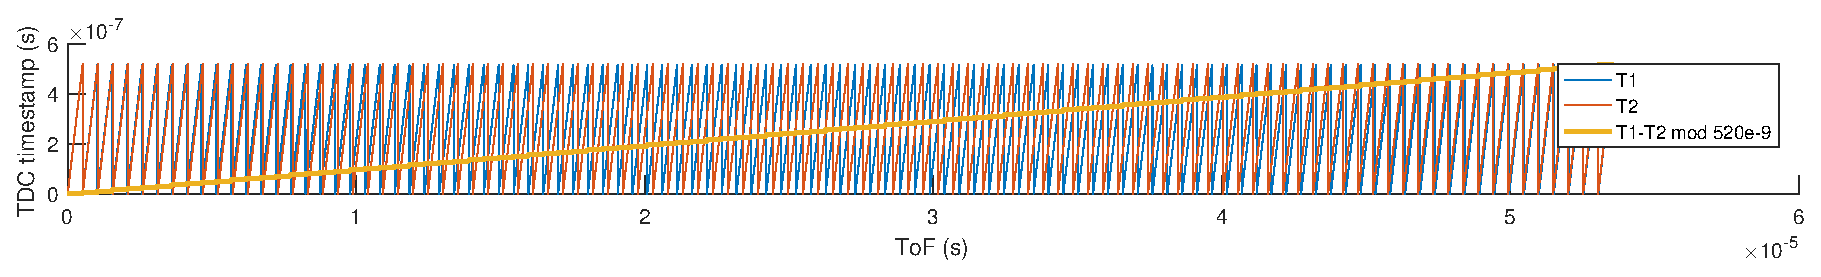
\includegraphics[width=\textwidth]{fig/frequency_hopping.eps}
    \caption{Matlab plot of TDC measurements vs ToF}
    \label{fig:frequency_hopping}
\end{figure}

The $ToF$ can be calculated using \cref{eq:ToF}.

\begin{align}
	t_{1-2} &= (t_1-t_2)\mod T_2\\
	ToF &= \frac{t_{1-2}}{T_2-T_1}T_1+\frac{t_1+t_2-t_{1-2}}{2}\label{eq:ToF}
\end{align}
where $t_1$ and $t_2$ are the timestamp measurements for $f_1$ and $f_2$ respectively. $t_{1-2}$ is the modulus of the time difference between $t_1$ and $t_2$.

\section{Optics}\label{ssec:optics}
The receiver optics are a good place to start of with, because the optics are not very dependent on results achieved in other areas. The optics have to transport as many desired photons, and as little unwanted photons to the active area on the SPADs as possible. All while having an acceptable depth of field. 

The most basic solution is a single lens with an aperture. The opacity of the lens can be calculated with the absorption of the lens material and f-number of the lens using \cref{eq:basic_opacity}.

\begin{align}\label{eq:basic_opacity}
\text{opacity} = \frac{1-\text{absorption}}{\text{f-number}^2}
\end{align}

 The performance of a possible configuration is shown in \cref{tab:basic_optics}

\begin{table}[H]
\centering
\caption{Performance of basic optics solution}
\label{tab:basic_optics}
\begin{tabular}{|l|r|}\hline
    \textbf{Basic Optics} & \\
    \hline 
    f-number & $2.00\, $ \\
    absorption & $5.00\,\%$ \\
    opacity & $23.75\, \%$ \\
    \hline 
\end{tabular}
\end{table}


\subsection{Improvements}
There are a couple of additions that can improve the performance of the optics. The first and essential one, is the use of a bandpass filter. The transmitted signal will have a very specific bandwidth of $850\,nm$. Using a narrow bandpass filter one can filter out an enormous part of the background noise. The filter will have an opacity of $50\,\%$ for the target wavelength.

The captured photons that hit the lens need to be guided to the active area of the SPADs. If the active area on the chip is very small, one can use microlenses to improve the effectiveness of the optics. A Microlens focuses light on a single SPAD on the chip. Two types of microlenses will be considered: a spherical lens, and a square shaped lens. The presence of microlenses poses a limitation of the main lens. The f-number must be relatively large. A higher f-number means a smaller aperture and therefore more loss of photons. A way of dealing with this problem is to use a second lens instead. An overview of the available options is shown in \cref{tkz:receiver_optics}

\begin{figure}[H]
    \centering


\resizebox{\linewidth*3/4}{!}{
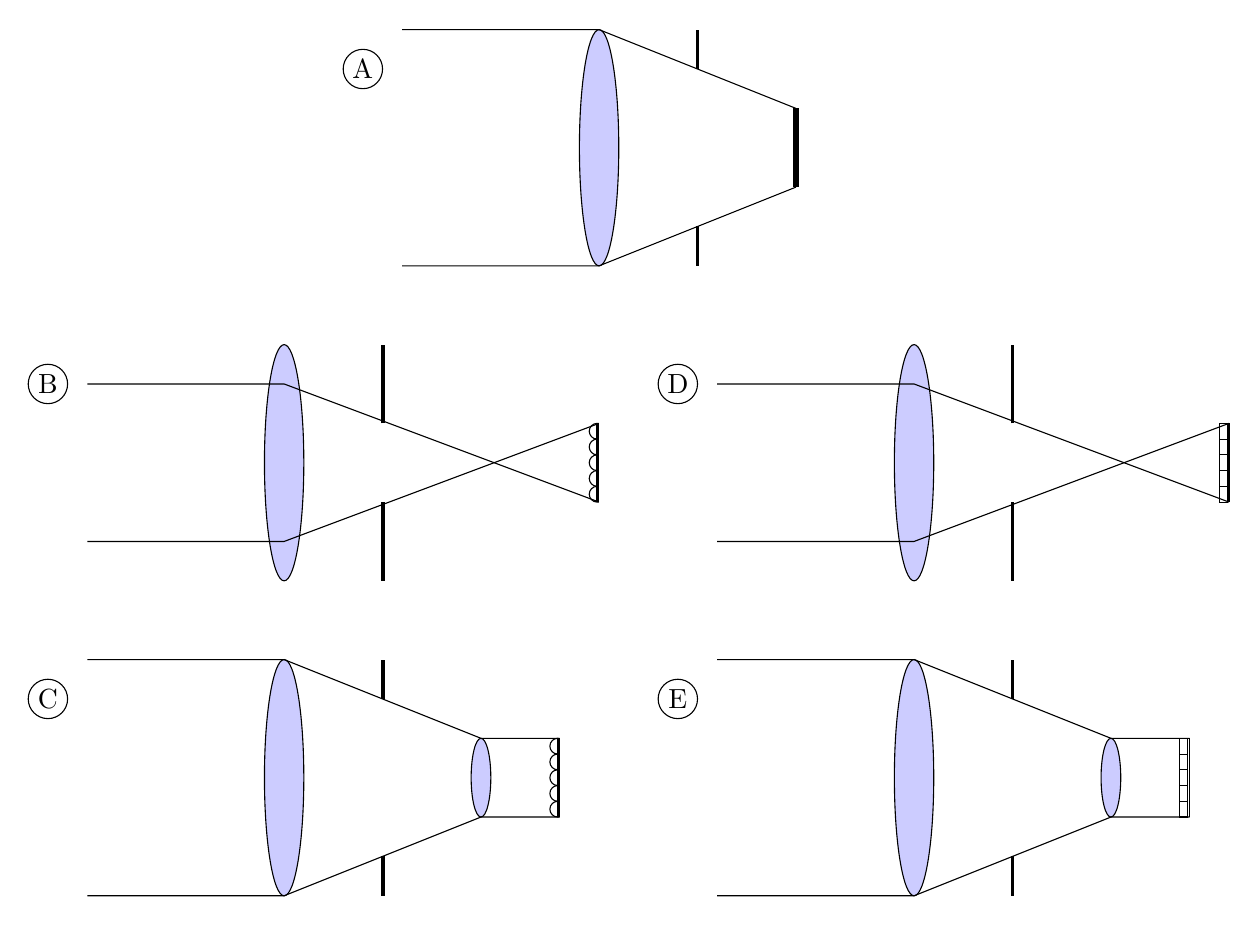
\begin{tikzpicture}[scale=.5]

%%%%%% low F-number, no microlens

%lens
\draw [fill=blue!20] (7,4) ellipse (0.5 and 3);

%diafragma
\draw [line width=.5mm] (9.5,6) -- (9.5,7);
\draw [line width=.5mm] (9.5,1) -- (9.5,2);

%sensitive area
\draw [line width=.7mm] (12,3) -- (12,5);

%light beams
\draw (2,7) to (7,7) to (12,5);
\draw (2,1) to (7,1) to (12,3);

%%%%%%Microlens + high F-number

%lens
\draw [fill=blue!20] (-1,-4) ellipse (0.5 and 3);

%diafragma
\draw [line width=.5mm] (1.5,-3) -- (1.5,-1);
\draw [line width=.5mm] (1.5,-7) -- (1.5,-5);

%sensitive area
\draw [line width=.7mm] (7,-5) -- (7,-3);

%light beams
\draw (-6,-2) to (-1,-2) to (7,-5);
\draw (-6,-6) to (-1,-6) to (7,-3) node (v1) {};


%Microlenses
\draw  (6.95,-3.2) ellipse (.2 and .2);
\draw  (6.95,-3.6) ellipse (.2 and .2);
\draw  (6.95,-4.0) ellipse (.2 and .2);
\draw  (6.95,-4.4) ellipse (.2 and .2);
\draw  (6.95,-4.8) ellipse (.2 and .2);
\fill  (7,-2.8) rectangle (7.4,-5.2) [fill=white];

%%%%%%Microlens + extra lens

%lens
\draw [fill=blue!20] (-1,-12) ellipse (0.5 and 3);

%second lens
\draw [fill=blue!20] (4,-12) ellipse (0.25 and 1);

%diafragma
\draw [line width=.5mm] (1.5,-10) -- (1.5,-9);
\draw [line width=.5mm] (1.5,-15) -- (1.5,-14);

%sensitive area
\draw [line width=.75mm] (6,-13) -- (6,-11);

%light beams
\draw (-6,-9) to (-1,-9) to (4,-11) to (6,-11);
\draw (-6,-15) to (-1,-15) to (4,-13) to (6,-13);


%Microlenses
\draw  (5.95,-11.2) ellipse (.2 and .2);
\draw  (5.95,-11.6) ellipse (.2 and .2);
\draw  (5.95,-12) ellipse (.2 and .2);
\draw  (5.95,-12.4) ellipse (.2 and .2);
\draw  (5.95,-12.8) ellipse (.2 and .2);
\fill  (6,-10.8) rectangle (6.4,-13.2) [fill=white];

%%%%%% Square Microlens + high F-number

%lens
\draw [fill=blue!20] (15,-4) ellipse (0.5 and 3);

%diafragma
\draw [line width=.5mm] (17.5,-3) -- (17.5,-1);
\draw [line width=.5mm] (17.5,-7) -- (17.5,-5);

%sensitive area
\draw  (23,-5) -- (23,-3);

%light beams
\draw (10,-2) to (15,-2) to (23,-5);
\draw (10,-6) to (15,-6) to (23,-3);


%Microlenses
\draw  (22.75,-3) rectangle (22.95,-3.4);
\draw  (22.75,-3.4) rectangle (22.95,-3.8);
\draw  (22.75,-3.8) rectangle (22.95,-4.2);
\draw  (22.75,-4.2) rectangle (22.95,-4.6);
\draw  (22.75,-4.6) rectangle (22.95,-5);


%%%%%% Square Microlens + extra lens

%lens
\draw [fill=blue!20] (15,-12) ellipse (0.5 and 3);

%second lens
\draw [fill=blue!20] (20,-12) ellipse (0.25 and 1);

%diafragma
\draw [line width=.5mm] (17.5,-10) -- (17.5,-9);
\draw [line width=.5mm] (17.5,-15) -- (17.5,-14);

%sensitive area
\draw  (22,-13) -- (22,-11);

%light beams
\draw (10,-9) to (15,-9) to (20,-11) to (22,-11);
\draw (10,-15) to (15,-15) to (20,-13) to (22,-13);


%Microlenses
\draw  (21.75,-11) rectangle (21.95,-11.4);
\draw  (21.75,-11.4) rectangle (21.95,-11.8);
\draw  (21.75,-11.8) rectangle (21.95,-12.2);
\draw  (21.75,-12.2) rectangle (21.95,-12.6);
\draw  (21.75,-12.6) rectangle (21.95,-13);



\draw  (1,6) ellipse (.5 and .5) node[]{A};
\draw  (-7,-2) ellipse (.5 and .5) node[]{B};
\draw  (-7,-10) ellipse (.5 and .5) node[]{C};
\draw  (9,-2) ellipse (.5 and .5) node[]{D};
\draw  (9,-10) ellipse (.5 and .5) node[]{E};


\end{tikzpicture}
}

    \caption{Overview of possible receiver optics implementations}
    \label{tkz:receiver_optics}
\end{figure}

\begin{align}
\text{opacity} = (1-\text{absorption}_1)(1-\text{absorption}_2)\cdot\text{opacity filter}\cdot \frac{X}{\text{f-number}^2}
\end{align}
Where $X$ is the active area on the chip. A comparison between the different options is shown in \cref{tab:receiver_optics}

\begin{table}[H]
\centering
\caption{comparison of different optics solutions}
\label{tab:receiver_optics}
\begin{tabular}{|l|lllll|}\hline
\textbf{Type}                & \textbf{A}        & \textbf{B}        & \textbf{C}        & \textbf{D}        & \textbf{E}        \\ \hline
absorption $1^{st}$ lens & 0.05     & 0.05     & 0.05     & 0.05     & 0.05     \\
f-number                 & 2        & 8        & 2        & 8        & 2        \\
absorption $2^{nd}$ lens & 0        & 0        & 0.05     & 0        & 0.05     \\
active area on chip      & 0.05     & 0.55     & 0.55     & 0.65     & 0.65     \\ \hline
effective opacity            & 0.011875 & 0.008164 & 0.124094 & 0.009648 & 0.146656 \\ \hline
\end{tabular}
\end{table}

The comparison in \cref{tab:receiver_optics} shows some good alternatives to the basic lens, if there is a need for it due to a small active area on the chip. However, most of the future calculations will focus on the basic model A.


\section{Scanning motion}\label{ssec:scanning_motion}
In \cref{ssec:SPADs}, it was concluded that a SPAD array with one SPAD per pixel is not feasible. Therefore a scanning motion is required. Possible scanning motions for different SPAD array configurations are shown in \cref{tkz:scanning_motions}. Note that the $2048\times1$ motion is in essence a special case of the $2048\times N$ motion, where exactly one row of pixels is observed at a time. The $M\times N$, with $M<2048$ and $N<2048$ needs a scanning motion in both $x$ and $y$ direction. This makes the scanning motion very complicated and unreliable. Therefore only the family of solutions with $2048\times N$ with $N<2048$ will be considered.


\begin{figure}[H]
    \centering
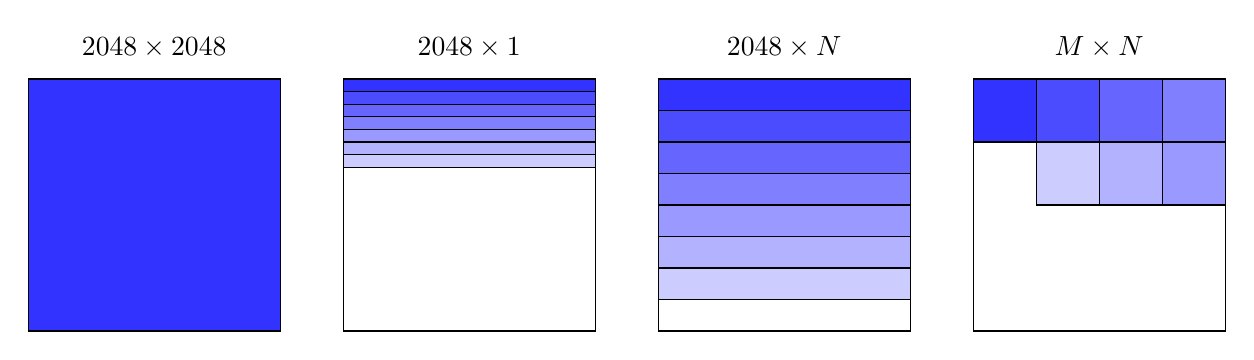
\begin{tikzpicture}[scale=.8]
\draw  (-3,4) rectangle (1,0);
\draw [fill=blue!80] (-3,4) rectangle (1,3.8);
\draw [fill=blue!70] (-3,3.8) rectangle (1,3.6);
\draw [fill=blue!60] (-3,3.6) rectangle (1,3.4);
\draw [fill=blue!50] (-3,3.4) rectangle (1,3.2);
\draw [fill=blue!40] (-3,3.2) rectangle (1,3);
\draw [fill=blue!30] (-3,3) rectangle (1,2.8);
\draw [fill=blue!20] (-3,2.8) rectangle (1,2.6);


\draw  (2,4) rectangle (6,0);
\draw [fill=blue!80] (2,4) rectangle (6,3.5);
\draw [fill=blue!70] (2,3.5) rectangle (6,3);
\draw [fill=blue!60] (2,3) rectangle (6,2.5);
\draw [fill=blue!50] (2,2.5) rectangle (6,2);
\draw [fill=blue!40] (2,2) rectangle (6,1.5);
\draw [fill=blue!30] (2,1.5) rectangle (6,1);
\draw [fill=blue!20] (2,1) rectangle (6,0.5);


\draw  (7,4) rectangle (11,0);
\draw [fill=blue!80] (7,4) rectangle (8,3);
\draw [fill=blue!70] (8,4) rectangle (9,3);
\draw [fill=blue!60] (9,4) rectangle (10,3);
\draw [fill=blue!50] (10,4) rectangle (11,3);
\draw [fill=blue!40] (10,3) rectangle (11,2);
\draw [fill=blue!30] (9,3) rectangle (10,2);
\draw [fill=blue!20] (8,3) rectangle (9,2);

\node at (-6,4.5) {$2048\times2048$};
\node at (-1,4.5) {$2048\times1$};
\node at (4,4.5) {$2048\times N$};
\node at (9,4.5) {$M\times N$};

\draw [fill=blue!80] (-8,4) rectangle (-4,0);
\end{tikzpicture}
    \caption{Different types of scanning motions}
    \label{tkz:scanning_motions}
\end{figure}


\subsubsection{Background Noise}\label{ssec:background_noise}
For the background noise, it is assumed that the sun is the dominant source. The sum is modelled as an ideal black body. The spectral irradiance of the sun can be calculated using \cref{eq:spectral_irradiance}.
\begin{align}\label{eq:spectral_irradiance}
I_\lambda(\lambda,T) = \frac{2hc^2}{\lambda^5}\frac{1}{e^{\frac{hc}{\lambda kT}}-1}
\end{align}
where $I_\lambda(v,t)$ is spectral irradiance with unit $W/m^3$. \\
$h$ is the planck constant\\
$c$ is the speed of light in vacuum \\
$k$ is the Boltzman constant \\
$\lambda$ is the wavelength of the electromagnetic radiation\\
$T$ is the absolute temperature of the body\\
The spectral irradiance of the sun is calculated in \cref{tab:sun_irradiance}.

\begin{table}[H]
\centering
\caption{Calculation of sun irradiation}
\label{tab:sun_irradiance}
\begin{tabular}{|l|ll|} \hline
\textbf{Sun irradiation} &          &                          \\ \hline
$h                        $&$ 6.63\cdot10^{-34} $&$ J\cdot s                 $\\
$c                        $&$ 3.00\cdot10^8     $&$ m/s                      $\\
$k                        $&$ 1.38\cdot10^{-23} $&$ j/K                      $\\
$\lambda                  $&$ 850               $&$ nm                         $\\
$T                        $&$ 5780              $&$ K                        $\\
$I_\lambda                $&$ 1.51\cdot10^{13}  $&$ W/m^3 $\\ \hline
\end{tabular}
\end{table}

The next step is to calculate the power emitted by the sun in the specified bandwidth, at the location of Europa. This is done by modelling sun as a point source, and then spreading that power over a sphere with a radius equal to the distance between the sun and Europa, as is done in \cref{eq:point_source}.

\begin{align}\label{eq:point_source}
    P_{sun} = I_{\text{sun}} B_\lambda S \frac{r_{\text{sun}}^2}{r_{\text{europa}}^2}
\end{align}
where $I_{\text{sun}}$ is the spectral irradiance of the sun at the center frequency of the filter, $B_\lambda$ is the bandwidth of the filter in meters, $S$ the surface area of the target area on Europa, $r_{\text{sun}}$ the of radius of the sun, and $r_{\text{europa}}$ the distance between Europa and the sun. The effective radiance of the background noise at Europa is calculated in \cref{tab:power_background} using \cref{eq:point_source}.

\begin{table}[H]
\centering
\caption{Effective power that hits the target area on Europa}
\label{tab:power_background}
\begin{tabular}{|l|ll|} \hline
\textbf{background power} &                     &         \\ \hline
$I_{lambda}$              & $1.51\cdot10^{13}$  & $W/m^3$ \\
$B$                       & $10$                & $nm$    \\
$S$                       & $15625$             & $m^2$   \\
$r_{sun}$                 & $695700$            & $m$     \\
$r_{europa}$              & $8\cdot10^8$        & $m$     \\
$P_B$                     & $0.179$             & $W$     \\ \hline
\end{tabular}
\end{table}
\subsection{Resolution} 
\label{ssec:resolution}
The requirement for the altimetry mode changes based on the height. The target is a resolution of at least $0.1\,\%$. To ensure that this requirement is met, both the largest altitude of $8\,km$, and the smallest altitude of $500\,m$ will be investigated.

The minimum resolution for the largest and shortest altitude are $8\,m$ and $0.5\,m$ respectively. The maximum allowable FWHM can be calculated using \cref{eq:max_FWHM}.
 Using \cref{eq:FWHM_sigma} the maximum standard deviation can be calculated. The calculations are performed

\begin{align}\label{eq:max_FWHM}
FWHM_{max} = \frac{2x}{c}
\end{align}

\begin{table}[H]
\centering
\caption{Required standard deviation to meet the system requirements}
\label{tab:AM_requirements}
\begin{tabular}{|l|rr|}\hline
    \textbf{AM requirements} & short & long \\
    \hline 
    altitude & $500\,m$ & $8\,km$ \\
    resolution & $50\,cm$ & $8\,m$ \\
    FWHM & $3.33\,n s$ & $53.33\,n s$ \\
    $\sigma$ & $1.42\,n s$ & $22.65\,n s$ \\
    \hline 
\end{tabular}
\end{table}








\subsubsection{standard deviation shortcut}
To calculate the standard deviation of the sum of multiple random variables that are independent and uncorrelated, one can use \cref{eq:variance_weighted_sum}


\begin{align}\label{eq:variance_weighted_sum}
\newcommand{\Var}{\mathrm{Var}}
 	\Var[aX+bY+cZ] = a^2\Var[X]+b^2\Var[Y]+c^2\Var[Z]
\end{align}




Next consider a situation where there are two random variable distributions. The first distribution is $S$, which is a normal distribution with $\mu_s=ToF$, where $ToF \in \{0, 50\mu\}$, and $\sigma_s=100p$. The second distribution is $N$, which is a uniform distribution with $\mu_n=\frac{50\mu}{2}$ and $\sigma_n=\frac{50\mu}{\sqrt{12}}$.

\begin{align}
	\mu_{mean} &= \frac{1}{110}\Big(\sum_{k=1}^{100}\mu_s+\sum_{l=1}^{10}\mu_n\Big)\\
			   &= \frac{100ToF+10*25\mu}{110}\\
			   &= \frac{10}{11}ToF+227.3n
\end{align}


\begin{align}
	\mathrm{Var}_{mean} &= \mathrm{Var}\Big[\frac{1}{110}\Big(\sum_{k=1}^{100}S_k+\sum_{l=1}^{10}N_l\Big)\Big]\\ 
	 &= \frac{1}{110^2}\Big(\sum_{k=1}^{100}\mathrm{Var}[S]+\sum_{l=1}^{10}\mathrm{Var}[N]\Big)\\
	&= \frac{1}{110^2}(100\sigma_s^2+10\sigma_n^2)\\
	&= \frac{10^{-18}+2.0833\cdot10^{-9}}{110^2}\\
	&= 1.7218\cdot10^{-13}\\
	\sigma_{mean} &= \sqrt{\mathrm{Var}_{mean}}\\
				  &= 414.94n
\end{align}



% Now we grab 100 samples out of $S$ and 10 out of $N$. First, the $\sigma$ and $\mu$ of the average of the 100 samples of $S$ is calculated.

% \begin{align}
% 	\mu_{s,mean} &= \frac{1}{100}\sum_{k=1}^{100}\mu_s\\
% 			     &= ToF
% \end{align}

% \begin{align}
% 	\mathrm{Var}[\frac{1}{100}\sum_{k=1}^{100}S_k] &= \frac{1}{100^2}\sum_{k=1}^{100} \mathrm{Var}[S_k]\\
% 						  &= \frac{\mathrm{Var}[S]}{100}\\
% 	\sigma_{s,mean} &= \frac{\sigma_s}{\sqrt{100}}\\
% 					&= 10p
% \end{align}

% Next the average of 10 samples of $N$ is calculated.

% \begin{align}
% 	\mu_{n,mean} &= \frac{1}{10}\sum_{k=1}^{10}\mu_n\\
% 			     &= 25\mu
% \end{align}

% \begin{align}
% 	\mathrm{Var}[\frac{1}{10}\sum_{k=1}^{10}] &= \frac{1}{10^2}\sum_{k=1}^{10} \mathrm{Var}[N_k]\\
% 						  &= \frac{\mathrm{Var}[N]}{10}\\
% 	\sigma_{s,mean} &= \frac{\sigma_n}{\sqrt{10}}\\
% 					&= \frac{50\mu}{\sqrt{120}}
% 					&\approx 4.5644\mu
% \end{align}

% Next the two resulting functions are combined






% \subsection{Laser}
The laser is responsible for the photons that are used for the Time of Flight (ToF) measurement. The laser has to ensure that the Signal to Background Noise Ratio (SBNR) is at least 0 dB. The power budget of the entire system is $50\,W$, which is the main bottleneck for the performance of the laser. The wavelength of the laser is $850\,nm$. The $P_B$ is already calculated in \cref{ssec:background_noise}. In order to achieve an SNR of 0 dB, the signal power $P_S$ must therefore at least match the background noise power that hits the surface of Europa. One can calculate the signal power at the optics using \cref{eq:P_S}.

\begin{align}\label{eq:P_S}
	P_S = P_{pulse} \cdot f_{pulse} \cdot R_{\text{Europa}}
\end{align}
where $P_{pulse}$ is the power of a single pulse of the laser, $f_{pulse}$ the frequency at which the pulses are transmitted, $R_{\text{Europa}}$ the reflectivity of Europa, and $r$ the altitude from the sensor to the surface of Europa. The SBNR can then be calculated using \cref{eq:SBNR}.

\begin{align}\label{eq:SBNR}
	SBNR &= \frac{P_S}{P_B}
\end{align}

The power of a single pulse can be calculated by combining \cref{eq:P_S} and \cref{eq:SBNR} into \cref{eq:p_pulse}. This is done in \cref{tab:p_pulse}.

\begin{align}
	P_{pulse} &= \frac{P_B\cdot SBNR}{f_{pulse}\cdot R_{\text{Europa}}}
\end{align}

\begin{table}[H]
\centering
\caption{Power of a laser pulse}
\label{tab:p_pulse}
\begin{tabular}{|l|ll|} \hline
\textbf{power of a laser pulse}  &              &      \\ \hline
$R_Europa$                       & $0.35        $&      \\
$P_B      $                      & $0.413       $&$ W/m^2 $\\
ground area coverage             & $15625       $&$ m^2   $\\
$SNBR      $                     & $0           $&$ dB   $\\
$f_{pulse}    $                    & $18750       $&$ Hz   $\\
$P_{pulse}     $                   & $0.3441 $&$ W    $\\ \hline
\end{tabular}
\end{table}

The $P_{pulse}$ is the optical power that is emitted by the laser. The electrical power is $\frac{P_{pulse}}{0.1}=3.4\,W$, which is well within the power envelope of $50\,W$. The next step is to calculate the required peak power $p_{peak}$ of the laser, using \cref{eq:p_peak}

\begin{align}\label{eq:p_peak}
 	P_{peak} &= \frac{P_{pulse}}{t_{pulse} \cdot f_{pulse}}
 \end{align} 
where $P_{peak}$ is the peak power and $t_{pulse}$ the FWHM of a pulse.

Using a typical pulse width of $t_{pulse} = 100\,ns$ and the $f_{pulse}$ as calculated in \cref{ssec:high_low_freq} one gets the result shown in \cref{tab:p_peak}.


\begin{table}[H]
\centering
\caption{Peak power calculation}
\label{tab:p_peak}
\begin{tabular}{|l|ll|} \hline
\textbf{Peak laser power} &             &    \\ \hline
$P_{pulse}                 $&$ 0.3441 $&$ W  $\\
$t_{pulse}                  $&$ 1.00\cdot10^{-7}    $&$ s  $\\
$f_{pulse}                  $&$ 18750       $&$ Hz $\\
$P_{peak}                  $&$ 184         $&$ W  $\\ \hline
\end{tabular}
\end{table}















%\clearpage
%\section{Overview} 
\label{sec:overview}

\begin{figure}[H]
    \centering



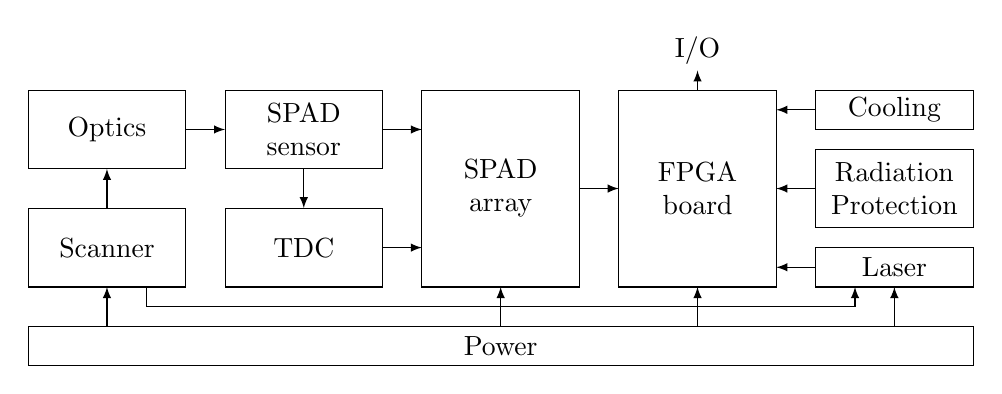
\begin{tikzpicture}[scale=.5]

\draw  (13,2) rectangle (17,1) node[pos=.5, align=center]{Cooling};
\draw  (13,0.5) rectangle (17,-1.5) node[pos=.5, align=center]{Radiation\\Protection};
\draw  (-7,-4) rectangle (17,-5) node[pos=.5, align=center]{Power};
\draw  (13,-2) rectangle (17,-3) node[pos=.5, align=center]{Laser};
\draw  (8,2) rectangle (12,-3) node[pos=.5, align=center]{FPGA\\board};
\draw  (3,2) rectangle (7,-3) node[pos=.5, align=center]{SPAD\\array};
\draw  (-2,2) rectangle (2,0) node[pos=.5, align=center]{SPAD\\sensor};
\draw  (-7,2) rectangle (-3,0) node[pos=.5, align=center]{Optics};
\draw  (-7,-1) rectangle (-3,-3) node[pos=.5, align=center]{Scanner};
\draw  (-2,-1) rectangle (2,-3) node[pos=.5, align=center]{TDC};

\draw [>=latex, ->](0,0) -- (0,-1);
\draw [>=latex, ->](2,-2) -- (3,-2);
\draw [>=latex, ->](13,1.5) -- (12,1.5);
\draw [>=latex, ->](7,-.5) -- (8,-.5);
\draw [>=latex, ->](2,1) -- (3,1);
\draw [>=latex, ->](13,-2.5) -- (12,-2.5);
\draw [>=latex, ->](10,2) -- (10,2.5);
\draw [>=latex, ->](-3,1) -- (-2,1);
\draw [>=latex, ->](13,-.5) -- (12,-.5);
\draw [>=latex, ->](5,-4) -- (5,-3);
\draw [>=latex, ->](10,-4) -- (10,-3);
\draw [>=latex, ->](15,-4) -- (15,-3);
\draw [>=latex, ->](-5,-1) -- (-5,0);
\node at (10,3) {I/O};

\draw [>=latex, ->](-5,-4) -- (-5,-3);
\draw [>=latex, ->](-4,-3) -- (-4,-3.5) -- (14,-3.5) -- (14,-3);

\end{tikzpicture}




    \caption{Schematic overview}
    \label{tkz:schematic_overview}
\end{figure}

\section{SPAD sensor} 
\label{sec:spad_sensor}
The SPAD Sensor generates a pulse when a photon is detected. It is connected to a TDC, and is used to construct a SPAD grid.

\subsection{requirements} 
\label{ssec:sensor_req}

\begin{table}[H]
    \begin{tabular}{l|l|l}
    ~                                  & Threshold & Goal \\ \hline
    Max Acquisition Slant Range        & 5 km      & 8 km \\
    Min Operational Range              & 5 m       & 1 m  \\
    Range Accuracy                     & 10 cm     & 5 cm \\
    Photon Detection Probability (PDP) & ?         & ?    \\
    Dead-time                          & ?         & ?    \\
    Dark count rate (DCR)              & ?         & ?    \\
    \end{tabular}
\end{table}

The most important requirement of the SPAD is the range accuracy of 5-10 cm. 

\begin{align*}
	\frac{5\cdot10^-2}{3\cdot10^8} &= 167\, ps 
\end{align*}

Therefore the jitter on the time between the arrival of a photon and the transmission of a pulse must be as small as possible.

\subsection{Possibilities} 
\label{ssec:sensor_pos}
To be continued

\subsection{Choice} 
\label{ssec:sensor_choice}
Basically we are going for CMOS Si SPAD's.


\section{TDC} 
\label{sec:tdc}
The Time intrerval to Digital Converted (TDC) is connected to a (or several) SPAD sensor. The TDC has to convert the difference in time between two pulses into a digital representation. It is used together with the SPAS sensors to build a SPAD grid.

\subsection{Requirements} 
\label{ssec:tdc_req}

\begin{table}[H]
    \begin{tabular}{l|l|l}
    ~                    & Threshold & Goal   \\ \hline
    accuracy             & 50 ps?    & 30 ps? \\
    jitter               & 30 ps?    & 10 ps? \\
    area per SPAD sensor & ?         & ?      \\
    power usage          & ?         & ?      \\
    \end{tabular}
\end{table}

\subsection{Possibilities} 
\label{ssec:tdc_pos}
There are a lot of possibilities here. But I don't know what technique they use to save on the amount of TDC's.

\subsection{Choice} 
\label{ssec:tdc_choice}


\section{SPAD grid} 
\label{sec:spad_grid}
The grid is the structure that implements the SPAD sensors and TDC's into a grid to measure 

\subsection{Requirements} 
\label{ssec:grid_req}

\begin{table}[H]
    \begin{tabular}{l|l|l}
    ~                                    & Threshold         & Goal              \\ \hline
    Update rate                          & 0.1 Hz            & 1 Hz              \\
    Ground Sample Distance               & 10 cm             & 5 cm              \\
    Ground Area Coverage at max altitude & 100 m times 100 m & 125 m times 125 m \\
    Time for 3D map creation             & 1 s               & 1 s               \\
    \end{tabular}
\end{table}

\subsection{Possibilities} 
\label{ssec:grid_pos}

\subsection{Choice} 
\label{ssec:grid_choice}
The unproposed master thesis board.

\section{FPGA board} 
\label{sec:fpga_board}

\subsection{Requirements} 
\label{ssec:grid_req}

\begin{table}[H]
    \begin{tabular}{l|l|l}
    ~                                    & Threshold         & Goal              \\ \hline
    Update rate                          & 0.1 Hz            & 1 Hz              \\
    Ground Sample Distance               & 10 cm             & 5 cm              \\
    Ground Area Coverage at max altitude & 100 m times 100 m & 125 m times 125 m \\
    Time for 3D map creation             & 1 s               & 1 s               \\
    \end{tabular}
\end{table}

Note that the relevant requirements are similar to the SPAD grid, because the SPAD grid has to generate the data, and the FPGA has to process it. 

\subsection{Possibilities} 
\label{ssec:grid_pos}

\subsection{Choice} 
\label{ssec:grid_choice}
The FPGA accompanying the unproposed master thesis board.

\section{Radiation protection} 
\label{sec:radiation_protection}

Because we cannot change the FPGA board to be more resilient against radiation. It  ight be necessary to protect the board with external components. 
\subsection{Requirements} 
\label{ssec:grid_req}

The FPGA has to survive a certain amounty of Cobalt-64 and proton radiation.

\subsection{Possibilities} 
\label{ssec:grid_pos}
The possibilities vary between different kinds of materials, different thickness, and positions. The possibility of no protection is also present.\\
\\


\subsection{Choice} 
\label{ssec:grid_choice}
The unproposed master thesis board.

\section{Laser} 
\label{sec:laser}



\chapter{Recommendations}\label{sec:recommendations}
This section contains the recommendations based on findings described in this report. The recommendations will be structured based on the rest of the document.

\section{Altimetry Mode Recommendations}
The calculations in \cref{sec:altimetry_mode} show that the Altimetry mode requires a focused laser and focused observation in order to be resource efficient. This might be achieved by turning of SPADs during the altimetry mode and sending a focused laser pulse. The performance can be further improved by using an intensity threshold to filter noise. Also the period of the laser, and the measurement time should be at least the maximum time of flight which is $53.3\,\mu s$. There is no need for complex optics. The Altimetry Mode is less critical than the Hazard Detection Mode. 

\section{Hazard Detection Mode}
Considering the required resolution and the size of a SPAD, it is not feasible to have a SPAD for every pixel. Therefore a $2048\times8$ grid is proposed. Depending on the achievable peak laser power, it is advantages to use very few pulses per measurement. A histogram with an intensity threshold is recommended to keep the required average and peak power within proportions. The histograms should be read out to the FPGA using a single bit serial shift register, where the intensity threshold is applied. The option to use a more sophisticated measurement method is worth consideration.

\section{Radiation}
The results from the radiation test are not in line with the expectation which means that extra investigation and confirmation is necessary to draw final conclusions about the technology. If the measured performance is representative for the performance it might be necessary to deliberately decrease the photon sensitivity of the chip to decrease the DCR and resilience against radiation of the SPADs. It might be worth considering using an older SPAD technology that has a proven resilience against radiation instead.



\appendix
\chapter{Double frequency sampling}
%-----------------------------------------
\subsubsection{Two frequency sampling}

The measurement time based on The maximum pulse frequency can then be calculated using \cref{eq:t_TDC_ToF}.  

\begin{align}\label{eq:t_TDC_ToF}
	t_{TDC} &=ToF \mod T_{pulse}\\	
	ToF &= t_{TDC}+k\cdot T_{pulse} & k \in \mathbb{N}\label{eq:ToF_t_TDC}
\end{align}


Where $t_{TDC}$ is the measurement of the TDC, $ToF$ the time of flight, and $T_{pulse}$ the time period of the laser pulses. The returned answer is related to $ToF$ as shown in \cref{eq:ToF_t_TDC}. There will be ambiguity when it is possible for $T_{pulse}$ to be smaller than $ToF$. The maximum frequency without ambiguity can be calculated using \cref{eq:pulse_f}.

\begin{align}\label{eq:pulse_f}
f_{pulse} = \frac{1}{t_{round}} = \frac{c}{2r}
\end{align}

To solve the ambiguity problem one can make measurements in two different frequencies. In the first half of the measurement, the pulses will have a period $t_1$, and in the second half a smaller period $t_2$. These two different measurements can first be used to determine the large scale ToF, and then the measurements can be combined to get a high accuracy to accompany that. The difference between the different measurements are in steps of equal distance. The size of these steps can be calculate with \cref{eq:t_step}.

\begin{align}\label{eq:t_step}
		t_{step} = t_1 - t_2
\end{align}

Given measurements $t_1$ and $t_2$ one can calculate the time of flight using \cref{eq:ToF}. 

\begin{align}
	t_{1-2} &= (t_1-t_2)\mod T_2\\
	ToF &= \frac{t_{1-2}}{T_2-T_1}T_1+\frac{t_1+t_2-t_{1-2}}{2}\label{eq:ToF}
\end{align}
where $t_1$ and $t_2$ are the timestamp measurements for $f_1$ and $f_2$ respectively. $t_{1-2}$ is the modulus of the time difference between $t_1$ and $t_2$.



\bibliographystyle{plain}
\bibliography{bib}{}

\end{document}


















